% Author :  Lionel du Peloux
% Contact : lionel.dupeloux@gmail
% Year : 2017
% !TEX encoding = UTF-8 Unicode

\chapter{Elastic rod~: equilibrium approach}
\label{chp:kirchhoff}

\section{Introduction}

In this chapter, following \citef{Dill1992}, we present thoroughly the theory of slender rods developed by Kirchhoff, Clebsch and Love at the end of the XIX\textsuperscript{th} century. This theory can be applied for motions where strains remain small although displacements may be large, which is perfectly suitable to the modeling of elastic gridshell structures where the material must be employed in its elastic range but the structure undergoes large displacements during the forming process.\footnote{This is classically referred to as \textquote{material linearity} but \textquote{geometric nonlinearity}. In the literature, \emph{large rotation} is also employed to refer to \emph{large displacement}.}

We will see that this theory requires nothing more than that, and that the shear strains are negligible. In particular, the rod is not supposed to be strictly inextensible, nor the cross-sections are assumed to remain strictly plane.

The discrete beam element presented in \cref{chp:numerical_model} will directly results from the discretization of the dynamical Kirchhoff equations presented here, combined with an appropriate use of the discrete curve-angle representation (see \cref{sec:crvangle}) and the circumscribed discrete curvature (see \cref{sec:circumscribed}).

The motivations for this work were build upon the experience gained in the previous chapter (see \cref{chp:energy}). Although the variational approach actually leads to the calculation of the quasi-static internal force and moment acting on the rod, these results are more straightforwardly obtained with the approach developed in this chapter, that is through writing the dynamic equilibrium of the rod. But it is not simply a matter of taste considering the perspective of the discrete element we intend to build and solve through a damped dynamic explicit time integration, namely a \emph{dynamic relaxation} procedure (see \cref{chp:numerical_model}). Indeed, the equilibrium approach enables an immediate and full dynamic treatment of the rod, drops the stiff and unnecessary constraint of inextensibility and naturally integrates the treatment of applied loads. It also offers a more physical and less mathematical understanding of the problem, which is a matter of concern when designing real structures.\footnote{The formalism of the energy formulation has it pros as it is more straightforwardly translated into minimization problems. Therefor, its resolution is naturally opened to a wide range of algorithm such as Newton-Raphson method, the conjugate gradient method, the steepest descent methods, \telp{}}

Finally, this approach is closer \textquote{in spirit} to what have been proposed previously in the field of active bending structures about the \dofs{3} or \dofs{6} \emph{spline beam} elements, and first introduced by \citef{Adriaenssens2001}. It brings a more robust background to explain how internal forces and moments are derived in those elements. For instance, in \cite{Adriaenssens2001,Douthe2006,DAmico2014} the unbalanced shear forces acting on the rod during its motion are deduced -- with no justification -- from the bending moment, itself computed from the curvature of the rod. We show here that this result is a consequence of the dynamic Kirchhoff equations where some inertial terms have been neglected (see \cref{sec:eq_of_motion}).



%
%Finally, 
%
%Moreover, in the field of bending active structures, 
%
%This chapter gives a more solid background to 
%
%
%This theory is valid for solids where one dimension is much larger than the two others and for motions
%
%Ici on explique que l'approche par les équations d'équilibre est beaucoup plus directe que l'approche énergétique.
%
%\footnote{For a shearable rod, the condition that $\vect{d}_3$ and $\vect{t}$ coincide is relaxed.}
%\footnote{in the directions of the principal axes of inertia of its cross-section}
%\footnote{The parameter $\rconf{s}$, usually chosen as the arc length parameter for the undeformed rod, is no longer the arc length parameter for the deformed rod, since there are deformations of shear and extension. The current arc length of the deformed rod is a function of $\rconf{s}$, which is often denoted by $s(\rconf{s})$.}
%
%
%\blockcquote[p.~xvii]{Benvenuto1991b}{The battle between weight and rigidity constitutes, in itself, the single aesthetic theme of art in architecture~: and to bring out this conflict in the most varied and clearest way is its office.}
%
%\blockcquote[p.~xvii]{Villaggio1997}{The theory of elastic structures is, by definition, the collection of all reasonable models, proposed during almost three centuries, concerned with simplifying the sol of problems involving elastic bodies. The equations describing the motion and equilibrium of a three-dimensional elastic body were formulated in full generality during the first half of the nineteenth century, but their solutions are known only in a few cases.}
%
%\blockcquote[p.~68]{Audoly2010}{In a deformed state, the center line has no particular reason to remain straight and, in general, $\vect{d}_1$ and $\vect{d}_2$ will twist along the center line. However, in the case of small strain that we consider, the triad $(\vect{d}_1,\vect{d}_2,\vect{d}_3)$ remains approximately orthonormal, provided it has been chosen orthonormal in the reference configuration. This is known as the Euler-Bernoulli or Navier-Bernoulli kinematical hypothesis, or sometimes the assumption of unshearable rods.}
%
%Extension to the case of thin-walled sections by~\cite{Dias2015, Vetyukov2014} in the case of ribbons. From the Vlasov
%
%\blockcquote[p.]{Dias2014}{For thin beams having a slender cross-section, $h \ll w$, the classical rod theory of Kirchhoff is known to be inapplicable. Such beams are usually modeled using Vlasov’s theory for thin-walled beams. Vlasov’s models can be justified from 3D elasticity but only in the case of moderate deformations, when the cross-sections bend by a small amount. In the present work, however, we have considered large deformations of thin strips. The strip has been modeled as an inextensible  plate, and the geometric  constraint of inextensibility has been treated exactly~: the cross-sections are allowed to bend by a significant amount. Our model extends the classical strip model of Sadowsky, and reformulate it in a way that fits into the classical theory of rods.}
%

\subsection{Overview}

We begin by a short introduction on the Cosserat theory of rods (see \cref{sec:cosserat_theory}). From this theory, we study only the way the motion of a rod is described in a very generic manner, through its force and moment strain vectors. We then restrain our study to the Kirchhoff theory of rods (see \cref{sec:kirchhoff_theory})~: we specialize the description inherited from the Cosserat theory to our needs so it fulfills the specific assumptions made in Kirchhoff theory~; we establish the dynamical equations of a rod under external loading~; we recall the canonical form of the strain and stress tensors~; and finally we retrieve the usual material constitutive equations as a consequence of the small strains and elasticity assumptions. Finally, we show that the static member of the equations of motion can be retrieved from simple geometric considerations (see \cref{sec:geointerp}).

\subsection{Contributions}
\begin{itemize}
\item We describe the motion of a Kirchhoff rod as a particular case of the motion of a Cosserat rod. This would enable to extend the present work in order to take into account shear effects, while sticking to the same geometrical description.
\item We retrieve the equations of motion of a Kirchhoff rod with a careful treatment of the assumptions, following \cite{Dill1992}.
\item We highlight the pedagogical interest of this approach compared to the variational approach by showing that the static members of Kirchhoff equations are nothing but first-order balance equations.
\end{itemize}

\subsection{Related work}

The theory for slender rods presented here was developed at the end of the XIX\textsuperscript{th} century by Kirchhoff \cite{Kirchhoff1850,Kirchhoff1876}, Clebsch \cite{Clebsch1883} and Love \cite{Love1906}.

\citef{Dill1992} revisits the work of these pioneers and treats their theory in the framework of modern continuum mechanics. He gives the dynamic equations of balance of momentum, with a careful and precise treatment of the assumptions. In particular, he makes the correct distinction between material and geometric curvatures, a subtlety that is often hidden behind the assumption that the beam is inextensible \cite{Adriaenssens1999,Douthe2007,DAmico2014}.\footnote{\blockcquote[p.~5]{Dill1992}{The principal normal, binormal, and torsion of the axis, viewed as an element of a space curve, have no special significance in the theory of rods. Use of those special directions as base vectors does not simplify the theory and can mislead the reader into attributing significance to them when none exists. In particular, the curvature of the rod should not be confused with the curvature of the space curve which the axis forms.}} His work is mentioned by \citef{Neukirch2009}. 


\citef{Timoshenko1921} proposes a theory that extends Kirchhoff, Clebsch and Love works to take into account shear effects, considering that cross-sections might not stay perpendicular to the centerline of the beam. For plane problems, he measures the amount of shear through a rotation of the cross-section with respect to the beam axis.

\citef{Reissner1973} and \citef{Simo1991} introduce the notion of \emph{geometrically exact} beam, that is a beam model in which the description of the geometry is free of any assumption. They derive generalized Kirchhoff equations for rods that can undergo stretching, shearing, bending, torsion and even warping in \cite{Simo1991} with the help of a 7\textsuperscript{th} degree of freedom. The problem is formulated from the principle of virtual work and is fully nonlinear, which means it accounts for both large-displacements and finite-strains. A similar attempt is proposed by \citef{Antman1974}. These formulations are nothing but two-director Cosserat theories in which the material frames is constrained to remain orthonormal, but not necessary adapted to the centerline.
 
\citef{Antman2005} develops the \emph{special theory of Cosserat rods}, a very generic theory applicable to the modeling of solids where one dimension is much larger than the other two. This theory is a generalization of the previous works of Antman, Reissner and Simo where the directors of the material frame are no more constrained to rigid body motions. Several authors interested in the modeling and simulation of nonlinear dynamics of rods built their work upon Antman's theory, among which we can cite \citef{Gregoire2007}, \citef{Spillmann2007} or \citef{Cao2008}.

\citef{Lang2009} claim that Lagrangian field theory leads to a more straightforward development of the work of Simo \cite{Simo1991} that is directly formulated using quaternions, which could be of practical interest when considering its implementation in a numerical solver.

\citef{Cisternas2002} extend Dill and Coleman extensible rod model to take into account thermal expansion. \citef{Moulton2013} offers an interesting treatment of extensible rods to model plants growth, whereas all the other papers cited here usually try to built their model upon the assumption that the rod is inextensible.

\citef{Lazaro2016} presents a review of geometrically exact models for very flexible rods with the prospect of modeling bending active structures.

%Pourquoi pas proposer une frise chronologique + un tableau de synthèse des hyptohèses.

\section{Introduction to the special Cosserat theory of rods}\label{sec:cosserat_theory}

This paragraph gives a very brief overview of the \emph{special Cosserat theory of rods}, as presented by~\citef{Antman2005}, that accounts for bending, torsion, extension and shear  behaviors of slender beams.\footnote{\blockcquote[p.~270]{Antman2005}{[we formulate] a general dynamical theory of rods that can undergo large deformations in space by suffering flexure, torsion, extension, and shear. We call the resulting geometrically exact theory the \emph{special Cosserat theory of rods}.}} This theory -- which is a \emph{director theory} of rods -- was first introduced by~\cite{Antman1974}. It gives a larger scope to the basements of the present work -- which relies on the \emph{Kirchhoff theory of rods} -- as the last is a special case of this larger theoretical framework. Thus, what is presented in this paragraph could be considered as a reasonable starting point to extend the present work, for instance to take account for shear deformations or large extensions, which might be relevant for some engineering problems or form-finding processes.

It has been largely employed in various fields~\cite{Shi1995, Bergou2010}.

\begin{figure}[p]
  	\begin{leftfullpage}
		\centering
     		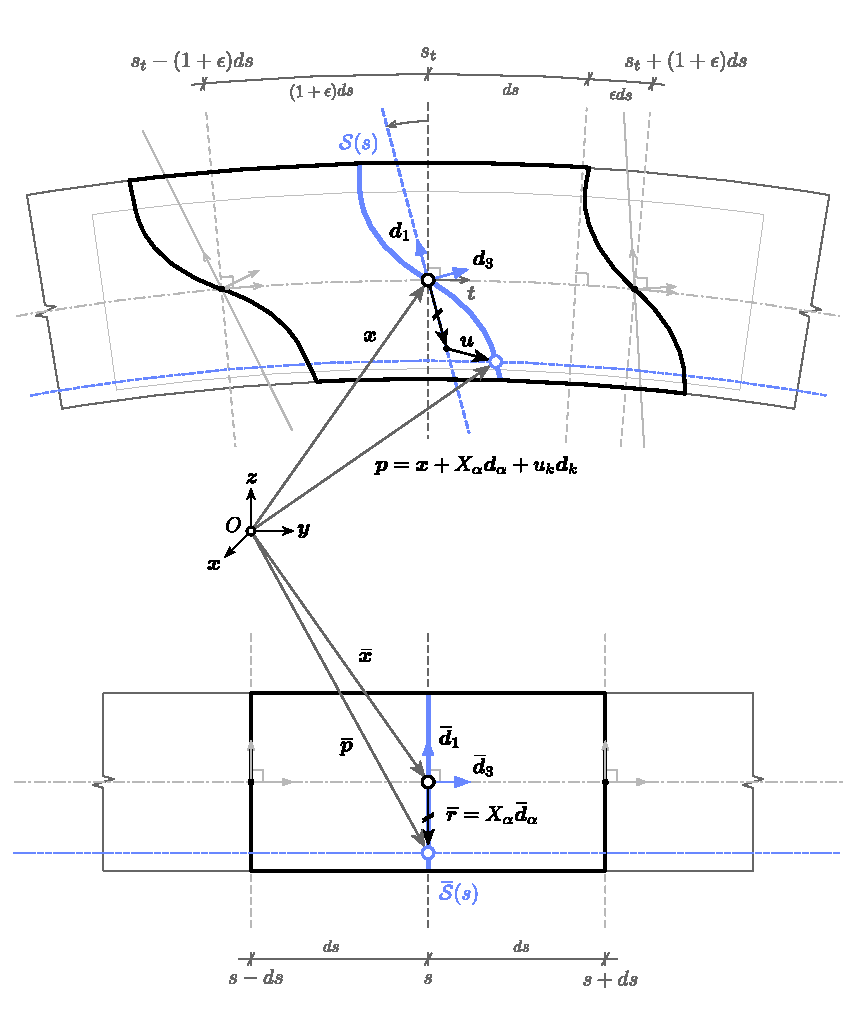
\includegraphics{cosserat_motion_longi.pdf}
		\captionof{figure}[Description of the motion for a Cosserat rod~: longitudinal section]{Description of the motion for a Cosserat rod. This is a typical longitudinal section of a rectangular beam deformed from a reference configuration (bottom) to an actual configuration (top) at time $t$. Cross-sections are defined in the reference configuration to be planar surfaces perpendicular to the beam axis ($\rconf{\mathcal{S}}$). A material point $\rconf{\vect{p}} \in \rconf{\mathcal{S}}(s)$ is located relatively to the cross-section centroid ($\rconf{\vect{x}}(s)$) thanks to its material coordinates ($X_1$, $X_2$, $s$). During the motion, this material point reaches a new position $\vect{p} \in \mathcal{S}(s)$. The deformed cross-section ${\mathcal{S}}(s)$ is no more planar. The material frame is no more aligned with the beam axis ($\vect{d}_3$ and $\vect{t}$ are not parallel any more). The actual position is measured from the centroid of the deformed cross-section ($\vect{x}(s)$) plus an in-plane component ($X_{\alpha}\vect{d}_{\alpha}$) and a deformation vector ($\vect{u}$). If the cross-sections deform in a rigid-body manner, then $\vect{u}$ is null everywhere.}
		\label{fig:cosserat_1}
	 \end{leftfullpage}
\end{figure}
\begin{figure}[p]
	\begin{fullpage}
		\captionsetup[subfloat]{captionskip=10pt}
     		\centering
     		\subfloat[][Deformed cross-section $\mathcal{S}(s)$]{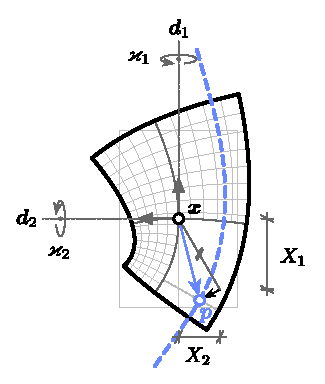
\includegraphics{cosserat_motion_trans_def_a.pdf}\label{fig:cosserat_2a}}
		\hspace{2.5cm}
		\subfloat[][Deformed cross-section $\mathcal{S}(s+ds)$]{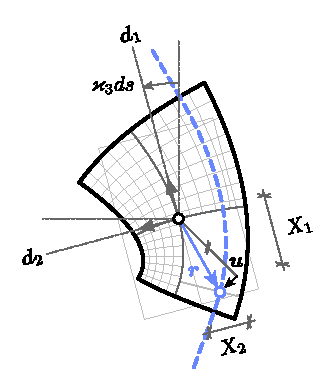
\includegraphics{cosserat_motion_trans_def_b.pdf}\label{fig:cosserat_2b}} \\
		\vspace{20pt}
		\subfloat[][Reference cross-section $\rconf{\mathcal{S}}(s)$]{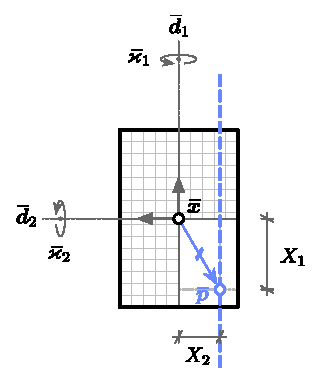
\includegraphics{cosserat_motion_trans_ref_a.pdf}\label{fig:cosserat_2c}}
		\hspace{2.5cm}
		\subfloat[][Reference cross-section $\rconf{\mathcal{S}}(s+ds)$]{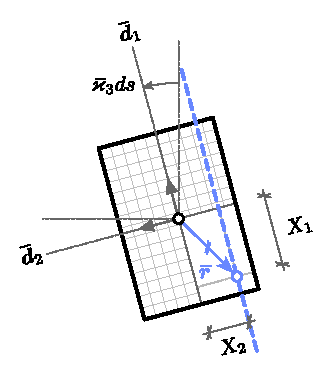
\includegraphics{cosserat_motion_trans_ref_b.pdf}\label{fig:cosserat_2d}}
		\vspace{20pt}
		\captionof{figure}[Description of the motion for a Cosserat rod: transverse section]{Description of the motion for a Cosserat rod. These are the transverse sections from \cref{fig:cosserat_1} (however note that \cref{fig:cosserat_1} is drawn with $\varkappa_2 < 0$ while $\varkappa_2 > 0$ in \cref{fig:cosserat_2}). The section curve is drawn in a dashed blue fashion. Remark how the deformed material point is located through $\vect{x}$ and $\vect{r} = X_{\alpha}\vect{d}_{\alpha} + u_{k}\vect{d}_{k}$. Cross-sections are rotating around $\vect{d}_3$ at speed $\varkappa_3$. The beam is subjected to flexion ($\varkappa_1 > 0$, $\varkappa_2 > 0$), torsion ($\varkappa_3 > 0$) and extension ($\epsilon > 0$). Fibers that are compressed -- both directly by axial compression or indirectly by flexion -- are subjected to transverse expansion due to the Poisson effect (see up-right of \cref{fig:cosserat_2a,fig:cosserat_2b}). Reciprocally, fibers in tension -- both directly by axial tension or indirectly by flexion -- are subjected to transverse contraction (see bottom-left of \cref{fig:cosserat_2a,fig:cosserat_2b}).}
		\label{fig:cosserat_2}    
	\end{fullpage}
\end{figure}

% Description of the motion
% ----------------------------------
\subsection{Description of the motion}\label{sec:cosserat_motion}
The special Cosserat theory of rods consider dynamics of rods. It relies on a precise geometric description (see \cref{fig:cosserat_1}) of rods build upon three vector-valued functions that are time dependent~: 
\begin{itemize}
\item
$\vect{x}$, a position vector describing the geometry in space of a specific \emph{fiber} called the rod \emph{axis} or \emph{centerline}. This function describes the rod in its longitudinal dimension. This dimension is of prime importance in the case of slender bodies such as rods as what is intend is to build a reduced theory, namely a 1-dimensional theory. This curve will often be understood as the curve passing through the cross-section centroids along the rod, although this is not mandatory in the theory.
\item
$\vect{d}_1$, $\vect{d}_2$, two unit vector fields describing the lateral spatiality of the rod and called material \emph{directors}. These vectors will often be understood as the principal axis of the cross-section, although this is not mandatory in the theory.
\end{itemize}
Modeling the geometry of the rod in any configuration is not sufficient to build a mechanical model. Indeed, one must know a \emph{reference} state for the solid as strains measure relative change in geometry and stresses are related to strains through the constitutive relation of the rod material. Thus, the special Cosserat theory of rods consider two configurations~:
\begin{itemize}
\item
The \emph{actual} configuration, that is the configuration of the rod at time $t$ during the motion.
\item
The \emph{reference} configuration, that is the configuration of the rod in a specific state where its geometry (possibly curved and twisted) is known and its mechanical state (strains, stresses) under possible loads (dead weight, temperature, wind, snow , prestress, \dots) and possible boundary conditions is known. In practice, this configuration will often be chosen as a \emph{stress-free} configuration when the beam is not subject to any loads nor restrains of any kind, although this is not mandatory in the theory.
\end{itemize}
Thus, the equations governing the motion of a \emph{special Cosserat rod} will be based on the description of a fully known reference configuration and the description of the actual or deformed configuration of the rod at time $t$ during its motion (see \cref{fig:cosserat_1}). Usually, what is intended is to predict the motion of a particular rod given its reference configuration, material properties, boundary conditions, and loading. In this thesis, the equations of the motion will be integrated to converged as fast as possible to the quasi-static response of the system, as this work only deals with statics of structures. However, it is still possible to use a more convenient and accurate time integrator to compute the motion, if  one wants to study the (true) dynamic of a rod and go beyond the knowledge of its static equilibrium.

Hereafter, when ambiguity is possible, symbols referring to the reference configuration will be marked with an overline while symbols referring to the actual configuration will be marked with a subscript in the variable $t$. Generally, scalar quantities are marked with the subscript $t$ and vector quantities with an overline in order to avoid double subscripts when one will refer to vector components.

\subsubsection{Actual configuration}

At time $t$, the \emph{actual} or \emph{deformed} configuration of the rod $\{{\vect{x}}, {\vect{d}_1}, {\vect{d}_2}\}$ is described by its \emph{centerline} $\gamma_t \in \mathcal{C}^1([0,{L}]\times \mathbb{R}^3)$, a regular space curve~: 
\begin{equation}
	\fonctionL{\gamma_t(t, \cdot)}{[0,{L}]}{\mathbb{R}^3}{{s}}{\vect{x}(t,{s})}
\end{equation}
and two perpendicular unit vector fields~: \footnote{Requiring that  $\vect{d}_1 \perp \vect{d}_2$ implies that the description of the motion is conveninent only for small in-plane stretching and shearing of the cross-section. This constrain can be relaxed to lead to an even more general theory, called the \emph{2-director Cosserat theory}.}
\begin{equation}
	\fonctionL{(\vect{d}_1,\vect{d}_2)(t, \cdot)}{[0,{L}]}{\mathbb{R}^3 \times \mathbb{R}^3}{{s}}{(\vect{d}_1(t,{s}), \vect{d}_2(t,{s})) \; / \; 
	\vect{d}_1(t,{s}) \cdot \vect{d}_2(t,{s}) = 0
	}
\end{equation}
In addition, we define a third unit vector field as~: 
\begin{equation}
	\vect{d}_3 = \vect{d}_1 \times \vect{d}_2
\end{equation}
Thus, the centerline is framed with the orthonormal moving frame $\{\vect{d}_3, \vect{d}_1, \vect{d}_2\}$. The unit vectors $\vect{d}_i(t,{s})$ are called \emph{material directors}.

Note that the centerline is parametrized by ${s}$ chosen to be the arc length parameter of the \emph{reference} configuration. It may not coincide with the arc length parameter of the \emph{actual} configuration denoted by $s_t = \Psi(t, s)=\Psi_t(s)$ as the rod may suffer elongation. $L$ denotes the length of the centerline in the reference configuration. The actual length of $\gamma_t$ is denoted by $L_t$ so that $s_t\in[0,L_t]$.

Finally, a material point $\vect{p}$ of the body is located relatively to the centerline with the help of the local position vector $\vect{r}$ such that (see \cref{fig:cosserat_2a,fig:cosserat_2b})~:
\begin{equation}
	\vect{p}(\rconf{\vect{r}},t) = \vect{x}(s,t) + \vect{r} \bigl( \vect{x}(s,t), \vect{d}_1(s,t) , \vect{d}_2(s,t), \rconf{\vect{r}}, t \bigr) 
\end{equation}
Note that in the above expression a material point is uniquely identified -- in a very generic manner -- by its local position in the reference configuration ($\rconf{\vect{r}} = \rconf{\vect{p}} - \rconf{\vect{x}}$).

\subsubsection{Reference configuration}
We now identify a \emph{reference} configuration of the rod $\{\rconf{\vect{x}}, \rconf{\vect{d}_1}, \rconf{\vect{d}_2}\}$ with centerline $\rconf{\gamma} \in \mathcal{C}^1([0,{L}]\times \mathbb{R}^3)$, a regular space curve. This time, $s$ is the arc length parameter of  $\rconf{\gamma}$, which leads to the important relation between $\rconf{\vect{x}}$ and the unit tangent vector $\rconf{\vect{t}}$ of $\rconf{\gamma}$ ~:
\begin{equation}
	\frac{d \rconf{\vect{x}}}{ds} = \rconf{\vect{t}} \quad,\quad \norm{\rconf{\vect{t}}} = 1
\end{equation}
In this configuration, we define a cross-section ${\mathcal{S}}(s)$ as the set of material points lying in the plane perpendicular to the centerline $\rconf{\gamma}$ at position $\rconf{\vect{x}}(s)$. By definition, it is a planar surface in the reference configuration. However this surface will not necessary remain planar in any other configuration. Moreover, and only for this configuration, it makes sense to choose the centerline as the curve passing through the cross-section centroids.

Finally, we call \emph{material coordinates} of point $\rconf{\vect{p}} \in {\mathcal{S}}(s)$ the triple $(X_3=s, X_1, X_2)$ such that (see \cref{fig:cosserat_2c,fig:cosserat_2d})~:
\begin{subequations}
	\begin{alignat}{2}
		&\rconf{\vect{p}}(\rconf{\vect{r}}) = \rconf{\vect{x}}(s) + \rconf{\vect{r}} \bigl(\rconf{ \vect{x}}(s), \rconf{\vect{d}_1}(s) , \rconf{\vect{d}_2}(s), X_1, X_2 \bigr) 
		\\
		 &\rconf{\vect{r}}(s, X_1, X_2) =  X_1 \rconf{\vect{d}_1} (s) + X_2 \rconf{\vect{d}_2}(s)
	\end{alignat}
\end{subequations}
We also identify a \emph{fiber} as the set of material points that share the same cross-section coordinates ($X_1$, $X_2$) all along the rod in the reference configuration.

\subsubsection{Clarification about the notations}
Remark that we sometimes decorate the reference configuration (with an overbar) and we sometimes decorate the actual configuration (with the subscript $t$). Although this could seem confusing to the reader, this is meant to produce the lighter notation possible to enhance readability.
\begin{itemize}
\item 
Thereafter, the equations will be written with respect to the arc length of the reference configuration. Hence, it was found preferable that $s$ refers to the arc length of the reference configuration and that $s_t$ refers to the arc length of the actual configuration.
\item 
As a consequence of the previous item, it was found more logical that $L$ refers to the length of the rod in the reference configuration and that $L_t$ refers to the length of the rod in the actual configuration.
\item
$(X_3, X_1, X_2)$ refers to the same point in all configurations. Hence, there is no need to distinguish the actual configuration from the reference configuration and we drop the overbar symbol for these quantities.
\item
${\mathcal{S}}(s)$ refers to the same set of points in all configurations. Hence, there is no need to distinguish the actual configuration from the reference configuration and we drop the overbar symbol for this quantity.
\end{itemize}





\subsection{Time evolution}
The evolution in time of the rod is simply given by the velocity of its centerline ($\dot{\vect{x}}$) and the  \emph{angular velocity vector} or \emph{spin vector} ($\vect{\omega}$) of its material directors~: 
\begin{subequations}
	\begin{alignat}{2}
		&\frac{\partial \vect{x}}{\partial t} (s,t)  = \dot{\vect{x}}  \label{eq:velocity_a}
		\\[0.5em]
		&\frac{\partial \vect{d}_k}{\partial t} (s,t)  = \dot{\vect{d}_k} = \vect{\omega}(s,t) \times \vect{d}_k(s,t) \label{eq:velocity_b}
	\end{alignat}
\end{subequations}
From now on, the derivative with respect to time is denoted with an overdot symbol.

\subsection{Force and moment strains}
To compare rod's configurations we introduce the \emph{force strain vector} ($\vect{\eta}$) and the \emph{moment strain vector} ($\vect{\varkappa}$)~:
\begin{subequations}
	\begin{alignat}{2}
		&\frac{\partial \vect{x}}{\partial s} (s,t)  =  \vect{x}'  = \vect{\eta}(s,t) \label{eq:Fstrain}
		\\[0.5em]
		&\frac{\partial \vect{d}_k}{\partial s} (s,t)  = \vect{d}'_k = \vect{\varkappa}(s,t) \times \vect{d}_k(s,t)  \label{eq:Mstrain}
	\end{alignat}
\end{subequations}
where the derivative with respect to $s$ is denoted with a prime symbol.

The components of $\vect{\eta} = \eta_k \vect{d}_k$ and $\vect{\varkappa} = \varkappa_k \vect{d}_k$ expressed in the material frame basis $\{\vect{d}_3, \vect{d}_1, \vect{d}_2\}$ can be interpreted as the classical engineering strains that lead to the engineering stresses.\footnote{For a complete interpretation, see~\cite[p.~285]{Antman2005} or~\cite[ch.~3]{Audoly2010}.}\textsuperscript{,}\footnote{Einstein's notation is employed here. For instance~: $\vect{\eta} = \eta_k \vect{d}_k = \eta_3 \vect{d}_3 + \eta_1 \vect{d}_1 + \eta_2 \vect{d}_2$.} In particular $\eta_3 = \vect{x}' \cdot (\vect{d}_1 \times \vect{d}_2)$ characterizes the change in volume of the body while $\eta_1$ and $\eta_2$ characterize the shear deformations ; $\varkappa_3$ is the material twist of the rod while $\varkappa_1$ and $\varkappa_2$ are the material curvatures of the rod.\footnote{Here, the term \textquote{material} is necessary as the material curvatures don't coincide with the geometric curvatures, although they are related one to each other. Precisely, the distinction originates in the fact that $s$ is not a unit-speed parametrization of the centerline in the actual configuration.}

Observe the symmetry of \cref{eq:velocity_a,eq:velocity_b} and \cref{eq:Fstrain,eq:Mstrain} regarding the parameters $s$ and $t$~: ($\dot{\vect{x}}$, $\vect{\omega}$) governs the time evolution of the material frame while ($\vect{x}'$, $\vect{\varkappa}$) governs the spatial evolution of the material frame along the centerline.

\subsubsection{Clarification about the notations}
Here we have chosen to follow the denomination introduced by Reissner in \cite{Reissner1973}. This denomination is closed to the one employed by Antman in \cite[p.~284]{Antman2005} where the components of $\vect{\eta}$ are called the \emph{strains} (aka the force strains) and the components of $\vect{\varkappa}$ are called the strain rates (aka the moment strains).\footnote{For an extensible rod, the derivative with respect to $s$ and $s_t$ are not equivalent. The prime notation stands only for the derivation with respect to $s$, the arc length parameter of the rod in the reference configuration.}

It is true that $\vect{\eta}$ and $\vect{\varkappa}$ expressed the geometric configuration of the rod with respect to the arc length of the reference configuration. This description is invariant under rigid boy motions. Indeed, with $\vect{\eta}$ and $\vect{\varkappa}$ given, one can rebuilt the geometry of the rod by solving the differential system of equations formed by \cref{eq:Fstrain,eq:Mstrain}. However it seems a little improper to call them \emph{strain} as this denomination is usually reserved to the components of the strain tensor which measure by how much a solid departs from its natural configuration and are dimensionless entries.

\subsubsection{Material versus geometric curvature}

It is worth to bring some lights in the notion of material versus geometric curvature.

\subsection{Parametrization of the centerline}
Recall that because the centerline of the reference configuration is parametrized by arc length, the unit tangent vector in this configuration is given by~:
\begin{equation}	
	\rconf{\vect{t}}(s) = \frac{d \rconf{\vect{x}}}{d s} (\rconf{s}) = \rconf{\vect{x}}'(s)
	\quad , \quad
	\norm{\rconf{\vect{x}}'} = 1
\end{equation}
In the deformed configuration, the centerline is still parametrized by $s$ which is no more an arc length parameter because the centerline has suffered stretch. Thus, the unit tangent vector in this configuration is given by~: \footnote{However, because $s_t$ is an arc length parameter of $\gamma_t$~: $\vect{t}(s,t) = \frac{\partial \vect{x}}{\partial s_t}(s,t)$.}
\begin{equation}	
	\vect{t}(s,t) = \frac{{\vect{x}}'(s,t)}{\norm{{\vect{x}}'(s,t)}}
	\quad , \quad
	\norm{\vect{x}'} = \norm{\vect{\eta}'} \neq 1
\end{equation}
We introduce $\epsilon$, the extension of the rod which characterizes the local change in length of the rod centerline, defined as~:
\begin{equation}	
	 \norm{\vect{\eta}'(s,t)} = \frac{\partial s_t}{\partial s}(s,t) = \Psi'(s,t) = 1 + \epsilon(s,t)
 \end{equation}
 
\subsubsection{Inextensibility}
The rod is said to be inextensible if $\epsilon = 0$ everywhere and at all time. In this case, $s$ is a valid arc length parameter for the centerline in every configurations. Later, we will restrict to the case of rods subjected to small extension, that is $\epsilon(t, s) \ll 1$.

\subsubsection{Reparametrization}
Although either $s$ and $s_t$ can be chosen as the third material coordinate to describe a rod, the definition of the material strains are given with respect to $s$ and not $s_t$. This is a matter of concern as the constitutive relations -- classically of the form $M=EI\kappa$,  $N=ES\epsilon$, $Q=GJ\tau$ -- relies upon material strains. Thus, in theses equations, what takes place is a derivation with respect to $s$ and not to $s_t$, which matters if the rod is not required to be inextensible.

\subsection{To go further}

The reader is invited to refer to~\cite{Antman2005} to get a deeper understanding of the \emph{Cosserat theory for rods}, in particular to see how the governing equations are derived. Here, only the geometric description of a Cosserat rod has been presented in a very generic but still concise manner. This description will be used in the next sections in the narrower scope of the (first order) \emph{Kirchhoff theory for rods} but could be usefully employed for richer theories. 

%\begin{figure}[p]
%\begin{fullpage}
%	\captionsetup[subfloat]{captionskip=20pt}
%     	\centering
%     	\subfloat[][Centerline of the discrete biarc model.]{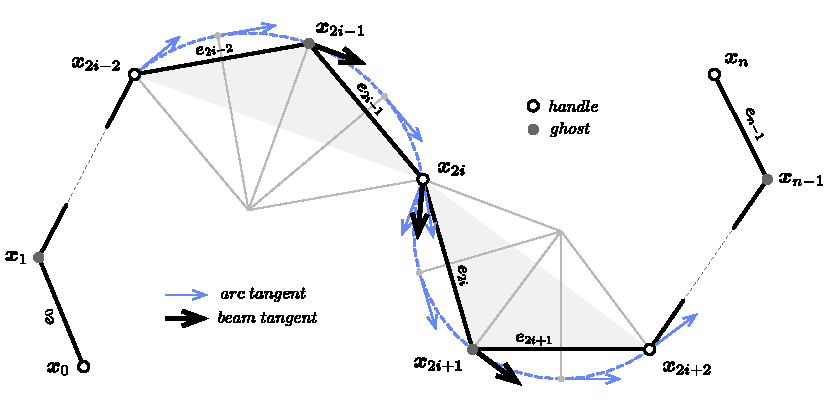
\includegraphics{discrete_model.pdf}\label{fig:discrete_model}} \\
%	\vspace{30pt}
%	\subfloat[][Number of segments, edges and vertices whether the centerline is closed or open.]{
%		\begin{tabular}{l  l | c  c } 
%		 &  & open & closed \\
%		\hline
%		segments & $n_s$ & $n_s$ & $n_s$ \\
%		\hline
%		edges & $n_e$ & $2 n_s$ & $2 n_s$ \\
%		\hline
%		vertices & $n$ & $2 n_s + 1$ & $2 n_s$ \\
%		\hline
%		ghosts & $n_g$ & $n_s$ & $n_s$ \\
%		\hline
%		handles & $n_h$ & $n_s+1$ & $n_s$ \\
%	\end{tabular}\label{tab:count}}
%	\vspace{20pt}
%	\caption{Biarc model for a discrete beam. The centerline is divided into curved segments (grey solid hatch). Each segment is defined as a three-noded element with uniform material and section properties. It has two end vertices (white) called \emph{handle} as they are used to interact with the model, for instance to apply loads or restrains. It has one mid vertex (grey) called \emph{ghost} as it is used only to enrich the segment kinematics and is not accessible to the end user.}
%\end{fullpage}
%\end{figure}


\begin{table}[p]
\begin{fullpage}
\center
		\ra{1.5}
		\begin{tabularx}{0.8\textwidth}{@{} X c c @{}}
		\toprule
		 				& reference configuration										& actual configuration
		\\ \midrule
		arc length 			& $s = \Psi_t^{-1}(s_t)$ 										& $s_t = \Psi_t(s)$
		\\
		length 			& $L$ 													& $L_t$
		\\
		centerline			& $\rconf{\gamma}$ 											& $\gamma_t$
		\\
		position vector		& $\rconf{\vect{x}}$ 											& ${\vect{x}}$
		\\
		material frame		& $\{\rconf{\vect{d}_3},\rconf{\vect{d}_1},\rconf{\vect{d}_2}\}$ 			& $\{\vect{d}_3,\vect{d}_1,\vect{d}_2\}$
		\\
		material coordinates	& $(s, X_1, X_2)$ 											& $(s, X_1, X_2)$
		\\
		force strains 		& $\rconf{\vect{\eta}}$ 										& ${\vect{\eta}}$ 	
		\\
		moment strains 	& $\rconf{\vect{\varkappa}}$ 									& ${\vect{\varkappa}}$
		\\
		spin vector 		& $\rconf{\vect{\omega}}$ 									& ${\vect{\omega}}$ 
		\\
		axial extension 		& $ \rconf{\epsilon} = 0$ 									& $\norm{\eta} = \Psi'_t(s) = 1 + \epsilon$		
		\\
		arc length derivative 	& $ \frac{\partial}{\partial s} \cdot = (\cdot)'	$						& $\frac{\partial}{\partial s_t} \cdot = (1 + \epsilon)^{-1} (\cdot)'$			
		\\
		time derivative 		& $ \frac{\partial}{\partial t} \cdot = \dot{(\cdot)}$						& $ \frac{\partial}{\partial t} \cdot = \dot{(\cdot)}$		
		\\
		\bottomrule	
	\end{tabularx}
	\label{tab:count}
	\vspace{10pt}
	\caption[Summary of the notations]{Summary of the notations employed throughout this section.}
\end{fullpage}
\end{table}

\clearpage
\section{Kirchhoff theory of rods}\label{sec:kirchhoff_theory}

In this section we recall the principles of Kirchhoff theory of rods and we treat its geometrical description with the framework presented in \cref{sec:cosserat_theory} from Cosserat's theory.\footnote{\blockcquote[p.~238]{Antman2005}{The classical elastic rod theory of Kirchhoff (1859), called the kinetic analogue, is is a special case of our rod theory [\dots]}.} Kirchhoff's theory accounts for finite displacements but small strains, which means that only geometric nonlinearities can be modeled. We will show in \cref{sec:constit} that in the framework of 3D elasticity it is precisely the assumption of small strains that leads to the well-known material constitutive laws.

Our goal is to present a clean theory that leads to the dynamical equations of Kirchhoff. These equations will then be discretize in the next chapter to build a discrete element suitable for the computation of elastic gridshells.

As reported by Dill, in the literature most of the assumptions presented as the Kirchhoff assumptions were in fact not made by Kirchhoff, Clebsch nor Love. Actually a \emph{Kirchhoff-Love} rod is a rod in which the deformed configuration differs only by \emph{small deformations} from a configuration that satisfies the \emph{Euler-Bernoulli} assumptions, that is~: cross-sections are plane, undeformed and perpendicular to the beam centerline.\footnote{\blockcquote[p.~18]{Dill1992}{Kirchhoff's theory can only apply to that class of problems for three dimensional bodies such that the loads on the sides are relatively small and slowly varying. The dominate mode of deformation must be a global bending and twisting with small axial extension. If there are substantial local variations in curvatures or substantial transverse shears, his theory of bending of rods will not provide a satisfactory first approximation.}}\textsuperscript{,}\footnote{\blockcquote[p.~1]{Coleman1993}{We discuss here the dynamical equations of a theory of elastic rods that is due to Kirchhoff and Clebsch. This properly invariant theory is applicable to motions in which the strains relative to an undistorted configuration remain small, although rotations may be large. It is constructed to be a first-order theory, i.e., a theory that is complete to within an error of order two in an appropriate dimensionless measure of thickness, curvature, twist, and extension.}}

Hence, a Kirchhoff rod does not presuppose that the centerline is inextensible -- but that the extension is small -- nor that cross-sections remain plane -- but that their warping deformation is small. These hypothesis, if strictly respected in the model, would not lead to the right expression of the torsion constant or the correct expression of the material curvatures.

But to what extent these deformations are considered small ? The answer is that Kirchhoff's theory is a complete \emph{first order} theory in the parameter $\alpha$~:
\begin{equation}
	\alpha = \sup_{s \in [0,L]} \{ h/L, \epsilon, h \norm{\vect{\varkappa}}, h\norm{\rconf{\vect{\varkappa}}} \}
\end{equation}
where $L$ is the rod length, $h$ is the characteristic width of the cross-section, $\epsilon$ is the axial extension, $\vect{\varkappa}$ and $\rconf{\vect{\varkappa}}$ are the vectors of material curvatures respectively in the deformed and unstressed configurations \cite{Dill1992,Coleman1993}.


%\footnote{\blockcquote[p.~15]{Dill1992}{There are no constitutive relations for $F_1$ or $F_2$. They are determined by the balance of momentum as in the elementary linear theory of bending of rods.}}

%For an historical review~:~\cite{Benvenuto1991a}. Short review of the history of 1D beam models~:\cite[p.~243]{Antman2005}

\subsubsection{Summary of the assumptions}
\begin{itemize}
\item The rod is slender.
\item The strains are small although the displacements might be large.
\item The shear strains are negligible.
\item The cross-section is free to warp.
\item The shear-center and the centroid of the cross-section are at the same location.
\item The material and cross-section properties vary slowly along the rod.
\end{itemize}
%
%\clearpage

% Description of the motion
% ----------------------------------
\subsection{Description of the motion}\label{sec:kirchhoff_motion}
To describe the motion of a Kirchhoff rod, we use the framework presented in \cref{sec:cosserat_motion} for Cosserat rods.\footnote{We use the notation employed by Antman in his \emph{special Cosserat theory of rods}~: \blockcquote[p.~270]{Antman2005}{The motion of a special Cosserat rod is defined by three vector-valued functions~: $ [s_1, s_2] \times \mathbb{R} \ni  (s,t) \mapsto \vect{r}(s,t), \; \vect{d}_1 (s,t), \; \vect{d}_2 (s,t) \in \mathbb{E}^3$}. However, somme specific assumptions will be made over the directors in the context of Kirchhoff's theory.} However, we restrict its scope by requiring that transverse shear strains are negligible quantities, which is one of the fundamental assumptions made by Kirchhoff in his theory~:
\begin{subequations}
	\begin{alignat}{3}
		&\eta_1 &&\simeq 0
		\\
		&\eta_2 &&\simeq 0
	\end{alignat}
\end{subequations}
As a consequence, the material frame remains adapted to the centerline. The rod is not supposed to be strictly inextensible. However, as strains are assumed to be small, the axial strain is supposed to be small itself ($\epsilon \ll 1$), which translates to~:
\begin{subequations}
	\begin{alignat}{3}
		&\eta_3(s,t) = 1+ \epsilon(s,t)
		\\
		&\vect{d}_3(s,t) = \vect{t}(s,t)
		\\
		&\vect{x}'(s,t) = (1+\epsilon) \vect{t}(s,t)
	\end{alignat}
\end{subequations}

\subsubsection{Stress-free configuration}
% --------------------------------------------------
We now consider a \emph{stress-free} configuration of the rod as the \emph{reference} configuration.\footnote{See~\cite[p.~20]{Audoly2010} for precisions when such a configuration may not exist.} The rod is described by its centerline $\rconf{\gamma}$ and its material frame $\{\rconf{\vect{d}_3}, \rconf{\vect{d}_1}, \rconf{\vect{d}_2}\}$. Again, a planar cross-section is defined as the set of material points lying in the plane perpendicular to $\rconf{\gamma}$ and passing through $\rconf{\vect{x}}(s)$. The material directors $\rconf{\vect{d}_1}$ and $\rconf{\vect{d}_2}$ are now chosen to be aligned with the principal axes of inertia of the cross-section.\footnote{In case of an axisymmetric section, any pair of perpendicular unit vectors lying in the cross-section plane will be valid.} Thus, $\rconf{\vect{d}_3} = \rconf{\vect{d}_1} \times  \rconf{\vect{d}_2}$ is normal to the plane of the cross-section and adapted to the centerline ($ \rconf{\vect{d}_3} =  \rconf{\vect{t}}$). Moreover, the centerline is chosen to be the curve passing through the cross-section centroids and is required to be at least a regular space curve, which means that its tangent is continuously defined.

For a sufficiently slender rod, the position of material point $\rconf{\vect{p}}$ that belongs to cross-section $\mathcal{S}(s)$ (see \cref{fig:cosserat_1,fig:cosserat_2a,fig:cosserat_2b}) is expressed through its material coordinates $(s, X_1, X_2)$ as~: \footnote{The lateral dimension of the rod must be smaller than its radius of curvature. Otherwise, this description would lead to self intersecting cross-sections.}
\begin{subequations}
	\begin{alignat}{2}
		&\rconf{\vect{p}}(s, X_1, X_2) &&= \rconf{\vect{x}}({s}) + \rconf{\vect{r}}(s, X_1, X_2)
		\\
		 &\rconf{\vect{r}}(s, X_1, X_2) &&=  X_1 \rconf{\vect{d}_1}(s) + X_2\rconf{\vect{d}_2} (s)
	\end{alignat}
\end{subequations}
Consequently, for each $s$ in the reference configuration, $({X_1}, {X_2})$ is a cartesian coordinate system for the plane $\mathcal{S}(s)$. In this system the local coordinates of the cross-section centroid are $(0,0)$. 

Finally, the cross-section is assumed to be bounded and the planar boundary curve is defined by the implicit equation~: $f_s(X_1,X_2) = 0$. It is also required that the shear center and the centroid of the cross-section are at the same location, otherwise one would require a more complex kinematic description of the rod.\footnote{Some details are given in the conclusion.}

\subsubsection{Deformed configuration}\label{sec:kirchhoff_deform_conf}
% --------------------------------------------------
We now examine the motion of a Krichhoff rod and we call \emph{deformed} configuration its actual configuration at time $t$. In this configuration the rod undergoes internal stresses under body loads, external loads and constrains. 

The deformed configuration of the rod at time $t$ is described by its centerline $\gamma_t$, its material frame $\{{\vect{d}_3}, {\vect{d}_1}, {\vect{d}_2}\}$ and a local displacement field $\vect{u}$. The centerline of the rod is deformed into the space curve $\gamma_t$ with position vector $\vect{x}$~: 
\begin{equation}
	\fonctionL{\gamma_t}{[0,{L}]}{\mathbb{R}^3}{s}{\vect{x}(s,t)}
\end{equation}
A material point $\rconf{\vect{p}}$ in the \emph{reference} configuration is transported to position $\vect{p}$ in the \emph{actual} configuration so that (see \cref{fig:cosserat_1,fig:cosserat_2c,fig:cosserat_2d})~:
\begin{subequations}
	\begin{alignat}{2}
		&\vect{p}(s, X_1, X_2, t) &&= \vect{x}(s,t) + \vect{r}(s, X_1, X_2, t)
		\\
		&\vect{r}(s, X_1, X_2, t) &&=  X_1 \vect{d}_1 (s,t) + X_2 \vect{d}_2 (s,t) + \vect{u}(s, X_1, X_2, t)
		\\
		&\vect{u}(s, X_1, X_2, t) &&=  u_k(s,X_1,X_2,t) \vect{d}_k (s, t)
	\end{alignat}
\end{subequations}
Although the cross-section $\mathcal{S}(s)$ is a planar surface in the reference configuration, it deforms to a non-planar surface in the actual configuration since $\vect{u} \neq \vect{0}$.\footnote{$\mathcal{S}(s)$ refers to the same set of material points in any configurations. Sometimes a distinction is made between $\rconf{\mathcal{S}}(s)$ and ${\mathcal{S}}(s)$ to highlight that the planarity of cross-sections is lost during the motion.} The components $(u_1, u_2, u_3)^T$ of the local displacement field expressed in the material frame basis are required to be small in Kirchhoff's theory of rods.\footnote{Note that this hypothesis is the one made by Kirchhoff and does not correspond to the well-known \emph{Euler-Bernoulli} or \emph{Navier-Bernoulli} assumption where the sections remain planar, undeformed and normal to the centerline during the rod deformation. In particular, torsion is responsible for the warping of cross-sections -- that is cross-sections don't remain planar during the motion -- and leads to a distinct value of the twist modulus. This is clearly stipulated in~\cite{Dill1992, Audoly2010} but is often treated with confusion in the literature.} In practice, as explained by~\cite{Dill1992} this means that the considered motions must satisfy~:
\begin{equation}
	\frac{u_k}{h} = O(\alpha)
	\quad , \quad
	\frac{\partial u_k}{\partial X_1} = O(\alpha)
	\quad , \quad
	\frac{\partial u_k}{\partial X_2} = O(\alpha)
	\quad , \quad
	\frac{\partial u_k}{\partial s} = O(\alpha^2)
\end{equation}
In this theory, the material frame in the reference configuration deforms in a rigid-body manner so that it remains orthonormal and aligned to the principal axes of the cross-section -- within an error $O(\alpha^2)$.\footnote{\blockcquote[p.~344]{Coleman1993}{[\dots] upon deformation, the principal axes of $\mathcal{S}(s)$ do remain normal to each other and to the rod axis, at least to within the approximations of the present theory, i.e., to within an error $O(\alpha^2).$}.} Remark that this is different than assuming that cross-sections deform in a rigid-body manner, which is known as the \emph{Euler-Bernoulli} hypothesis and is equivalent to the special case $\vect{u} = \vect{0}$.

\subsection{Reparametrization}
% -------------------------------------------
This subsection highlights the role played by the change in length of the rod during its motion. It was found that this aspect is often treated partially or with confusion in the literature, although it is of prime importance to understand correctly the influence of axial stretch in the computation of moment strains. Indeed, for an inextensible rod, the notions of geometric curvature and (flexural) material curvatures are somehow the same notions. But this is not the case for extensible rods as explained in \cref{sec:kirchhoff_strains}.



The rod is parametrized by $s$, the arc length parameter of the \emph{reference} configuration, as the constitutive laws will be expressed relatively to this configuration. But recall once again that $s$ is no more the arc length parameter of the \emph{deformed} centerline as the rod may have suffer axial extension.\footnote{In Kirchhoff's theory, rods are not supposed to be strictly inextensible but extension has to remain small. Thus, the internal axial force is given by a constitutive law and not considered as a geometric constrained. However, some authors have remarked that it might be convenient and reasonable to solve the equations of motion considering the geometric contraint $\epsilon = 0$. See~\cite[p.~98]{Audoly2010} for a detailed discussion of the subject.} Kirchhoff's theory assumes that the material frame remains adapted to the centerline during deformation, or equivalently that transverse shear strains are neglected.\footnote{This is also known as the \textquote{unsherable} assumption. Indeed, if $\frac{\partial \vect{x}}{\partial s} = \eta_k \vect{d}_k = (1 + \epsilon)\vect{d}_3 \Leftrightarrow \eta_1 = \eta_2 = 0$.} The extension of the centerline is characterized by $\epsilon$ defined such that~:
\begin{subequations}
	\begin{alignat}{2}
		&\rconf{\vect{x}}' = \rconf{\vect{d}_3}
		\\
		&\vect{x}' = (1 + \epsilon) \vect{d}_3
	\end{alignat}
\end{subequations}
However, one can parametrized the deformed centerline by its own arc length parameter, denoted $s_t$. Let's call $L_t$ the length of the deformed centerline and $\Psi_t$ the $\mathcal{C}^1$ diffeomorphism that maps $s$ onto $s_t$ ($s_t = \Psi_t(s) \Leftrightarrow s = \Psi_t^{-1}(s_t)$). Thus, the centerline is equivalently described by~:
\begin{equation}
	\fonctionL{\gamma_t}{[0,{L_t}]}{\mathbb{R}^3}{s_t}{\vect{x}(s_t)}
\end{equation}
Because $s_t$ is the arc length parameter of $\gamma_t$ the following relations hold~:
\begin{subequations}
	\begin{alignat}{2}
		&\frac{\partial \vect{x}}{\partial s_t} &&= \vect{d}_3
		\\[0.5em]
		&\frac{\partial s_t}{\partial s} &&= \eta_3 = 1+ \epsilon
	\end{alignat}
\end{subequations}
Consequently, one can deduced that the derivation with respect to $s$ is proportional to the derivation with respect to $s_t$ by a factor $1 + \epsilon$. This factor has to be taken into account when computing the material curvatures, which are no more equivalents to their geometric counterparts in the deformed configuration. This is detailed in the next section dedicated to the force and moment strain vectors.

% Strains
% ----------
\subsection{Force and moment strains}
\label{sec:kirchhoff_strains}
This section, introduces the material force and moment strains vectors of a Kirchhoff rod. It shows how they are related -- yet distinct if $\epsilon \neq 0$ -- to the geometric curvature of the centerline.
\subsubsection{Reference configuration}
% --------------------------------------------------
Since the material frame is orthonormal and adapted to the centerline, its evolution along the undeformed centerline is described thanks to the \emph{reference material curvature vector} $\rconf{\vect{\varkappa}}$ defined as~:
\begin{equation}
	\rconf{\vect{d}_i}' = \rconf{\vect{\varkappa}}  \times \rconf{\vect{d}_i}
\end{equation}
In the reference configuration, because $s$ is the centerline's arc length parameter, the strains vector components expressed in the material frame basis take the form~: \footnote{Recall the following result for an adapted frame~: \cref{eq:amf_kb}.}
\begin{subequations}
	\begin{alignat}{4}
		&\rconf{\varkappa}_3 &&=  \rconf{\vect{d}_1}'  \cdot \rconf{\vect{d}_2} &&= \rconf{\tau} &&= \rconf{\vect{d}_1}'  \cdot \rconf{\vect{d}_2}
		\\
		&\rconf{\varkappa}_1 &&=\rconf{ \vect{d}_3}'  \cdot \rconf{\vect{d}_2} &&= \rconf{k}_1 &&= \rconf{\vect{\kappa b}} \cdot \rconf{\vect{d}_1}
		\\
		&\rconf{\varkappa}_2 &&= \rconf{\vect{d}_1}'  \cdot \rconf{\vect{d}_3} &&= \rconf{k}_2 &&= \rconf{\vect{\kappa b}} \cdot \rconf{\vect{d}_2}
	\end{alignat}
\end{subequations}
where $\rconf{\vect{\kappa b}}$ (see \cref{eq:kb}) is the curvature binormal vector of $\rconf{\gamma}$ ~:
\begin{equation}
 	\rconf{\vect{\kappa b}} =  \rconf{\vect{t}} \times  \frac{\partial \rconf{\vect{t}}}{\partial s} = \rconf{\vect{t}} \times \rconf{\vect{t}}'
\end{equation}
$\rconf{\varkappa}_1$ and $\rconf{\varkappa}_2$ are called the reference \emph{material} curvatures. $\rconf{\varkappa}_3$ is called the reference \emph{material} twist. In this configuration, $\rconf{\varkappa}_1$ and $\rconf{\varkappa}_2$ are simply computed as the projection of the curvature binormal vector along $\rconf{\vect{d}_1}$ and $\rconf{\vect{d}_2}$.

Note the important distinction between the reference material twist ($\rconf{\tau}$) and the torsion of Frenet ($\tau_f$) of the centerline, as defined in \cref{sec:ff}.

\subsubsection{Deformed configuration}
% --------------------------------------------------
Since the material frame is orthonormal and adapted to the centerline, it's evolution along the \emph{deformed} centerline is described thanks to the \emph{actual} moment strain vector ${\vect{\varkappa}}$ defined as~:
\begin{equation}
	\frac{\partial \vect{d}_k}{\partial s} =  \vect{d}'_k = {\vect{\varkappa}}  \times \vect{d}_k
\end{equation}
Note that the strains vector is defined relatively to the arc length $s$ of the \emph{reference} configuration and not the arc length $s_t$ of the \emph{actual} configuration. Thus the strains vector components expressed in the material frame basis are given by~:
\begin{subequations}
	\begin{alignat}{3}
		&{\varkappa}_1 &&= \vect{d}'_3  \cdot \vect{d}_2 &&= (1+\epsilon) {k_1} = (1+\epsilon)\, \vect{\kappa b} \cdot \vect{d}_1
		\\[0.5em]
		&{\varkappa}_2 &&= \vect{d}'_1  \cdot \vect{d}_3 &&= (1+\epsilon) {k_2} = (1+\epsilon)\, \vect{\kappa b} \cdot \vect{d}_2
		\\[0.5em]
		&{\varkappa}_3 &&=  \vect{d}'_1  \cdot \vect{d}_2 &&= (1+\epsilon) {\tau} = (1+\epsilon)\, \frac{\partial \vect{d}_1}{\partial s_t}  \cdot \vect{d}_2
	\end{alignat}
\end{subequations}
where $\vect{\kappa b}$ (see \cref{eq:kb}) is the curvature binormal vector of $\gamma_t$ given by~:
\begin{equation}
 	\vect{\kappa b} =  \vect{t} \times  \frac{\partial \vect{t}}{\partial s_t} = (1+\epsilon)\, \vect{t} \times \vect{t}'
\end{equation}
${\varkappa}_1$ and ${\varkappa}_2$ are called the \emph{material} curvatures. ${\varkappa}_3$ is called the \emph{material} twist. Note this time the dependence of the material moment strains $(\varkappa_3,\varkappa_1,\varkappa_2)$ regarding the extension of the rod. These are the strains employed in the classical constitutive laws that lead to the determination of the internal axial force ($N = ES \epsilon$), internal bending moments ($M_1 = EI_1(\varkappa_1-\rconf{\varkappa}_1)$, $M_2 = EI_2(\varkappa_2-\rconf{\varkappa}_2)$) and internal twisting moment ($Q = GJ((\varkappa_3-\rconf{\varkappa}_3)$). 

Often in the literature the flexural material curvatures are computed as the projection of the curvature binormal vector onto the first two material axes. Here it is demonstrated that this is not exact as it omits the contribution of the rod extension, although it could be a reasonable approximation when $\epsilon \ll 1$. 

% Balance of momentum
% ------------------------------
\subsection{Balance of momentum}
\begin{figure}[t]
	\centering
	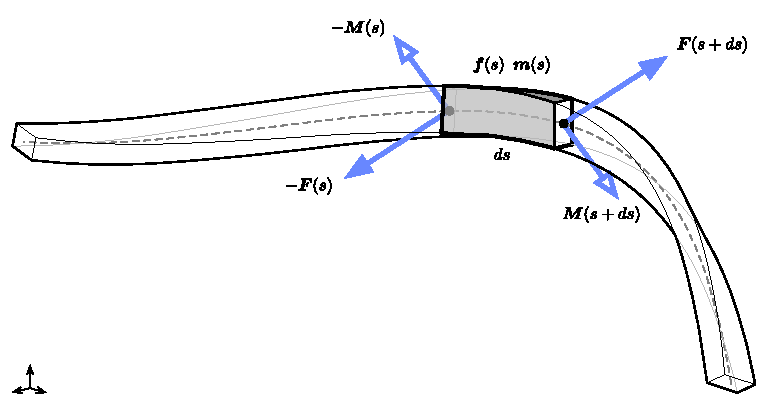
\includegraphics[]{kirchhoff_law.pdf}
	\captionof{figure}[Equilibrium of an infinitesimal slice of rod.]{Internal forces ($\vect{F}$) and moments ($\vect{M}$) acting on an infinitesimal beam slice of length $ds$. The beam is also subject to distributed external forces ($\vect{f}$) and moments ($\vect{m}$). By convention, internal forces and moments are forces and moments applied by the right part to the left part of the beam.}
	\label{fig:rodslice}
\end{figure}
Let $\vect{\mathcal{P}}$ be the first \emph{Piola-Kirchhoff} stress tensor. $\vect{\mathcal{P}}$ expresses how contact forces are acting in a \emph{deformed} body, referring to its (known) \emph{reference} configuration. Let $\vect{dS} =  \vect{n}dS$ be an elementary oriented surface of the rod in the \emph{reference} configuration, of centroid $\vect{p}(s,X_1,X_2,t) \in \mathcal{S}(s)$.\footnote{$dS$ is the area and $\vect{n}$ is the unit normal of the elementary oriented surface $\vect{dS}$.} The contact forces exerted on $\vect{dS}$ are given by~:
\begin{subequations}
	\begin{alignat}{2}
		&\vect{dF}(s,X_1,X_2,t) &&=  \vect{\sigma_n}(s,X_1,X_2,t) \,dS 
		\\
		&\vect{\sigma_n}(s,X_1,X_2,t) &&= \vect{\mathcal{P}}(s,X_1,X_2,t) \cdot \vect{n} \label{eq:piola}
	\end{alignat}
\end{subequations}
The \emph{Piola stress vector} ($\vect{\sigma_n}$) introduced in \cref{eq:piola} expresses the contact forces exerted on the body per unit area of the \emph{reference} configuration.\footnote{For a detailed introduction to the Piola-Kirchhoff stress tensor, refer to~\cite[p.~52]{Audoly2010}.}

The generic laws for the balance of linear and angular momentums are obtained by summation over the reference configuration, where $\vect{b}$ are the body forces per unit volume of the \emph{reference} configuration~:
\begin{subequations}
	\begin{alignat}{2}
		&\iiint_{\mathcal{V}} \rho \ddot{\vect{p}} \;dV 
		&&= \iint_{\partial\mathcal{V}} \vect{\sigma_n} \;dS 
		+ \iiint_{\mathcal{V}} \rho \vect{b} \;dV
		\label{eq:linearbalance}
		\\[0.5em]
		&\iiint_{\mathcal{V}} \rho (\vect{p} \times \ddot{\vect{p}}) \;dV  
		&&=  \iint_{\partial\mathcal{V}} \vect{p} \times \vect{\sigma_n} \;dS 
		+ \iiint_{\mathcal{V}} \rho (\vect{p} \times \vect{b}) \;dV
		\label{eq:angularbalance}
	\end{alignat}
\end{subequations}
Here, and subsequently, $\mathcal{V}$ denotes the volume of a slice of the rod in the \emph{reference} configuration, encompassed between two cross-sections ($\mathcal{S}_1 = \mathcal{S}(s_1)$, $\mathcal{S}_2 = \mathcal{S}(s_2)$, $s_1 < s_2$). We also denote $\mathcal{L}_{12}$ the lateral surface of the rod in the \emph{reference} configuration so that the exterior surface of the volume is~: $\partial \mathcal{V} = \mathcal{S}_1 \bigcup \mathcal{L}_{12} \bigcup \mathcal{S}_2$.

The cross-section $\mathcal{S}(s)$ splits the rod in two parts. Hereafter, the downstream part of the rod over $[s,L]$ will be called the \textquote{right part}. Reciprocally, the upstream part of the rod over $[0,s]$ will be called the \textquote{left part}.

\subsubsection{Internal forces and moments}
At the cross-section $\mathcal{S}(s)$, the contact forces applied by the right part onto the left part of the rod yield the following resultant force $\vect{F}$ and resultant moment $\vect{M}$ about the centroid point $\vect{x}(s,t)$~:
\begin{subequations}
	\begin{alignat}{2}
		&\vect{F}(s, t) &&= \iint_{\mathcal{S}(s)} \vect{\sigma_n}(s, X_1, X_2, t) \;dX_1 dX_2 \label{eq:F}
		\\[0.5em]
		&\vect{M}(s, t) &&= \iint_{\mathcal{S}(s)} \vect{r}(s,X_1,X_2,t) \times \vect{\sigma_n}(s, X_1, X_2, t) \;dX_1 dX_2 \label{eq:M}
	\end{alignat}
\end{subequations}
$\vect{F}$ and $\vect{M}$ are commonly known as the \emph{internal forces} and the \emph{internal moments} of the rod.

\subsubsection{External forces and moments}
We assume that the resultant of the contact forces on $\mathcal{L}_{12}$ and the body forces on $\mathcal{V}$ reduce to the following forms~:
\begin{subequations}
	\begin{alignat}{5}
		&\iint_{\mathcal{L}_{12}} \vect{\sigma_n} \;dS 
		&&+ \iiint_{\mathcal{V}} \rho \vect{b} \;dV
		&&= \int_{s_1}^{s_2} \big[\vect{f}_s  + (1+\epsilon) \vect{f}_{s_t} \big] \;ds
		\label{eq:f}
		\\[0.5em]
		&\iint_{\mathcal{L}_{12}} \vect{p} \times \vect{\sigma_n} \;dS 
		&&+ \iiint_{\mathcal{V}} \rho (\vect{p} \times \vect{b}) \;dV
		&&= \int_{s_1}^{s_2} \big[ \vect{m}_{s}  + (1+\epsilon) \vect{m}_{s_t}  \nonumber
		\\ & && &&\quad + \vect{x} \times \left(\vect{f}_{s}  + (1+\epsilon) \vect{f}_{s_t} \right) \big] \;ds
		\label{eq:m}
	\end{alignat}
\end{subequations}
where $\vect{f}_{s} $  (resp. $\vect{f}_{st}$) is the distributed resultant force per unit length of the reference (resp. deformed) configuration ; and $\vect{m}_{s} $  (resp. $\vect{m}_{s_t} $) is the distributed resultant moment per unit length of the reference (resp. deformed) configuration. For instance, these distributed forces and moments include external and body loads such as weight, snow, wind, \dots \footnote{At this stage, although this is uncommon in the literature, it has been found convenient to mark the distinction between loads referring to the reference configuration and loads referring to the actual configuration. Indeed, various distributed loads depend on the actual length of an element such as pressure and wind loads. On the other hand, some loads are independent of the extension of the rod, such as its weight.}

Note that Kirchhoff's theory require that the stress components on the sides of the rod are small~\cite[p.~11]{Dill1992} -- that is $\vect{\sigma_n}\cdot \vect{n} = O(\alpha^2)$ over $\mathcal{L}_{12}$. Thus, the first two terms in the above expression will be neglected~:
\begin{subequations}
	\begin{alignat}{2}
		&\iint_{\mathcal{L}_{12}} \vect{\sigma_n} \;dS \simeq 0
		\\[0.5em]
		&\iint_{\mathcal{L}_{12}} \vect{p} \times \vect{\sigma_n} \;dS \simeq 0
	\end{alignat}
\end{subequations}
Although the continuous model does not account formally for punctual loads,\footnote{This is possible but would require more math. However, local effects of such loads would not be properly modeled in the theory of Kirchhoff (Saint-Venant's Principle).} they will be introduced seamlessly in the discrete model as the dynamical equations for the motion of the rod will translate into rigid body equations for the discrete segments composing the rod.

\subsubsection{Inertial forces}
The inertial forces for a volume of the rod encompassed between cross-sections $\mathcal{S}_1$ and $\mathcal{S}_2$ are obtained by summation as~: 
\begin{subequations}
	\begin{alignat}{2}
		&\iiint_{\mathcal{V}} {\rho} \ddot{\vect{p}} \;dV = \iiint_{\mathcal{V}_t} {\rho_t} \ddot{\vect{p}} \;dV_t \label{eq:inertial_a}
		\\[0.5em]
		&\iiint_{\mathcal{V}} \rho (\vect{p} \times \ddot{\vect{p}}) \;dV= \iiint_{\mathcal{V}_t} {\rho_t} (\vect{p} \times  \ddot{\vect{p}}) \;dV_t \label{eq:inertial_b}
	\end{alignat}
\end{subequations}
Here, ${\rho}$ (resp. ${\rho_t}$) is the mass density of the rod in the reference (resp. deformed) configuration. Expressions are given in both coordinate systems.\footnote{In~\cite{Dill1992} the change in volume and the conservation of mass is expressed through the determinants of the metric tensors of the reference and deformed configurations. Recall that this determinant is the square of the volume of the elementary cell defined by $\frac{\partial \rconf{\vect{p}}}{\partial s}$, $\frac{\partial \rconf{\vect{p}}}{\partial X_1}$, $\frac{\partial\rconf{\vect{p}}}{\partial X_2}$ in the reference configuration, which is convected to the elementary cell defined by $\frac{\partial \vect{p}}{\partial s}$, $\frac{\partial \vect{p}}{\partial X_1}$, $\frac{\partial \vect{p}}{\partial X_2}$ in the reference configuration.}

In the context of Kirchhoff's approximation, the local deformations ($u_k$) of the cross-sections can be neglected in the computation of the inertial forces~\cite[p.~16]{Dill1992}. This yields~:
\begin{subequations}
	\begin{alignat}{2}
		&\vect{p} &&\simeq \vect{x} + X_1\vect{d}_1 + X_2\vect{d}_2
		\\
		&\dot{\vect{p}} &&= \dot{\vect{x}} + \vect{\omega} \times (X_1\vect{d}_1 + X_2\vect{d}_2)
		\\
		&\ddot{\vect{p}} &&= \ddot{\vect{x}} + \dot{\vect{\omega}} \times (X_1\vect{d}_1 + X_2\vect{d}_2) + \vect{\omega} \times ( \vect{\omega} \times (X_1\vect{d}_1 + X_2\vect{d}_2))
	\end{alignat}
\end{subequations}
Since $X_1$ and $X_2$ are the coordinates with respect to the centroid ($\vect{x}$) and the principal axes of the cross-section ($\vect{d}_1$, $\vect{d}_2$), the cross-section area ($S$) and principal moments of inertia ($I_1$, $I_2$) are given by~: \footnote{This is exact in the reference configuration but only approximately true in the deformed configuration as the theory consider only small deformations of cross-sections.}\textsuperscript{,}\footnote{\cref{eq:centroid_a} is nothing but the definition of the centroid position. \cref{eq:diag} holds because the tensor of inertia of the cross-section is diagonal in the basis $\{\vect{d}_3, \vect{d}_1, \vect{d}_2\}$ and thus $I_{12} = I_{21} = 0$.}
\begin{subequations}
\label{eq:sectionprop}
	\begin{alignat}{2}
		&0  		&&= \iint_{\mathcal{S}(s)} \left(X_1 X_2\right) \;dX_1 dX_2 \label{eq:diag}
		\\
		&S 		&&= \iint_{\mathcal{S}(s)} dX_1 dX_2
		\\
		&I_1 		&&= \iint_{\mathcal{S}(s)} {X_2}^2 \;dX_1 dX_2
		\\
		&I_2 		&&= \iint_{\mathcal{S}(s)} {X_1}^2 \;dX_1 dX_2
		\\
		&I_p 		&&= \iint_{\mathcal{S}(s)} ({X_1}^2 + {X_2}^2) \;dX_1 dX_2
	\end{alignat}
\end{subequations}
Moreover, for a given cross-section the definition of the centroid yields~:
\begin{subequations}
\label{eq:centroid}
	\begin{alignat}{2}
		&\vect{0}  &&= \iint_{\mathcal{S}(s)} \left(X_1\vect{d}_1 + X_2\vect{d}_2\right) \;dX_1 dX_2 \label{eq:centroid_a}
		\\
		&0 		&&= \iint_{\mathcal{S}(s)} {X_1} \;dX_1 dX_2 \label{eq:centroid_b}
		\\
		&0 		&&= \iint_{\mathcal{S}(s)} {X_2} \;dX_1 dX_2 \label{eq:centroid_c}
	\end{alignat}
\end{subequations}
For a thin slice of the rod ($\delta\mathcal{V}$) between cross-sections $\mathcal{S}(s)$ and $\mathcal{S}(s+ds)$, \cref{eq:inertial_a,eq:inertial_b} yield respectively~: \footnote{Indeed, since $\iint_{\mathcal{S}(s)} \vect{r} \;dX_1 dX_2 = \vect{0}$ from \cref{eq:centroid_a} we have $\iint_{\mathcal{S}(s)} \ddot{\vect{r}} \;dX_1 dX_2 =  \iint_{\mathcal{S}(s)} \dot{\vect{\omega}} \times \vect{r} + \vect{\omega} \times ( \vect{\omega} \times \vect{r}) \; dX_1 dX_2 = \vect{0}$ and $\iint_{\mathcal{S}(s)} \vect{r} \times \ddot{\vect{x}} \; dX_1 dX_2 = \vect{0}$ as $\vect{\omega}$ and $\vect{x}$ are independent of $X_1$ and $X_2$.}
\begin{subequations}
	\begin{alignat}{2}
		&\iiint_{\delta\mathcal{V}} {\rho} \ddot{\vect{p}} \;dV= ({\rho}S \ddot{\vect{x}})ds
		\\[0.5em]
		&\iiint_{\delta\mathcal{V}} \rho (\vect{p} \times \ddot{\vect{p}}) \;dV= \left({\rho}S \ddot{\vect{x}} + {\rho} \iint_{\mathcal{S}(s)} \vect{r} \times \ddot{\vect{r}} \; dX_1 dX_2 \right)ds
	\end{alignat}
\end{subequations}
Finally, remark that~:
\begin{equation}
	\vect{r} \times \ddot{\vect{r}}
	= (X_1)^2 \vect{d}_1 \times \ddot{\vect{d}_1} 
	+ (X_2)^2 \vect{d}_2 \times \ddot{\vect{d}_2} 
	+ X_1 X_2 (\vect{d}_1 \times \ddot{\vect{d}_2} 
	+ \vect{d}_2 \times \ddot{\vect{d}_1})
\end{equation}
Thus, reminding \cref{eq:sectionprop,eq:centroid}, one can conclude that the inertial forces reduce to~:
\begin{subequations}
	\begin{alignat}{2}
		&\iiint_{\delta\mathcal{V}} {\rho} \ddot{\vect{x}} \;dV= ({\rho}S \ddot{\vect{x}})ds \label{eq:linearinertia}
		\\[0.5em]
		&\iiint_{\delta\mathcal{V}} \rho (\vect{p} \times \ddot{\vect{p}}) \;dV = ({\rho}S \ddot{\vect{x}} + \rho I_1 \vect{d}_1 \times \ddot{\vect{d}_1} + \rho I_2 \vect{d}_2 \times \ddot{\vect{d}_2}) ds \label{eq:angularinertia}
	\end{alignat}
\end{subequations}

\subsubsection{Balance of linear momentum}
For a thin slice of the rod ($\delta\mathcal{V}$) between cross-sections $\mathcal{S}(s)$ and $\mathcal{S}(s+ds)$, using \cref{eq:F,eq:f}, the balance of linear momentum referring to the \emph{reference} configuration expressed in \cref{eq:linearbalance} yields~: 
\begin{equation}
	\begin{aligned}
		\iiint_{\delta\mathcal{V}} \rho \ddot{\vect{p}} \;dV 
		&= \iint_{\partial\mathcal{V}} \vect{\sigma_n} \;dS 
		+ \iiint_{\delta\mathcal{V}} \rho \vect{b} \;dV
		\\[0.5em]
		&= \iint_{\mathcal{S}(s)} \vect{\sigma_n} \;dS 
		+ \iint_{\mathcal{S}(s+ds)} \vect{\sigma_n} \;dS
		+ \left( \iint_{\delta\mathcal{L}} \vect{\sigma_n} \;dS
		+ \iiint_{\delta\mathcal{V}} \rho \vect{b} \;dV \right)
		\\[0.5em]
		&= -\vect{F}(s) + \vect{F}(s+ds) + \big(\vect{f}_{s} (s) + (1+\epsilon) \vect{f}_{s_t}(s) \big) ds
		\\[0.5em]
		&= \left( \frac{\partial \vect{F}}{\partial s} + \vect{f}_{s}  + (1+\epsilon) \vect{f}_{s_t} \right)(s) ds
	\end{aligned}
\end{equation}
Thus, using \cref{eq:linearinertia}, the equation for the balance of linear momentum reduce to~: \footnote{This equation also writes~: $(1+\epsilon)\frac{\partial \vect{F}}{\partial s_t} + \vect{f}_{s}  + (1+\epsilon)\vect{f}_{s_t} = \rho S \ddot{\vect{x}}$.}
\begin{equation}
	\frac{\partial \vect{F}}{\partial s} + \vect{f}_{s}  + (1+\epsilon)\vect{f}_{s_t} = \rho S \ddot{\vect{x}}
	\label{eq:linearmotion}
\end{equation}

\subsubsection{Balance of angular momentum}
Similarly, for a thin slice of the rod ($\delta\mathcal{V}$) between cross-sections $\mathcal{S}(s)$ and $\mathcal{S}(s+ds)$, using \cref{eq:F,eq:M} yields~: 
\begin{alignat}{5}
	\iint_{\mathcal{S}(s) \bigcup \mathcal{S}(s+ds)} \vect{p} \times \vect{\sigma_n} \;dS
	&= \iint_{\mathcal{S}(s) \bigcup \mathcal{S}(s+ds)} (\vect{x} + \vect{r}) \times \vect{\sigma_n} \;dS 
	\\[0.5em]
	&= -(\vect{x}\times\vect{F})(s) + (\vect{x}\times\vect{F})(s+ds) - \vect{M}(s) + \vect{M}(s+ds) \nonumber
	\\[0.5em]
	&=  \frac{\partial}{\partial s} \big( \vect{M} + \vect{x}\times\vect{F} \big)(s) ds \nonumber
\end{alignat}
Using \cref{eq:m} the balance of linear momentum referring to the \emph{reference} configuration expressed in \cref{eq:angularbalance} yields~: 
\begin{alignat}{5}
	\label{eq:angularbalance2}
	&\iiint_{\delta\mathcal{V}} \rho (\vect{p} \times \ddot{\vect{p}}) \;dV  
	&&=  \iint_{\partial\delta\mathcal{V}} \vect{p} \times \vect{\sigma_n} \;dS 
	+ \iiint_{\delta\mathcal{V}} \rho (\vect{p} \times \vect{b}) \;dV
	\nonumber \\[0.5em]
	& &&= \frac{\partial}{\partial s} \big( \vect{M} + \vect{x}\times\vect{F} \big)(s) ds 
	+ \vect{m}_{s}  + (1+\epsilon)\vect{m}_{s_t}  \\
	& &&\quad + \vect{x} \times \big(\vect{f}_{s}  + (1+\epsilon)\vect{f}_{s_t} \big) \;ds \nonumber
\end{alignat}
Finally, combining \cref{eq:angularbalance2} with \cref{eq:linearmotion,eq:angularinertia}, the equation for the balance of angular momentum reduce to~: \footnote{Note the simplification of the term $\rho S \ddot{\vect{x}}$. Alternatively, the balance equations could be written for the slice considered as a rigid body. In the barycentric frame of the slice~: $\frac{d}{dt}(dI_G) = \vect{M}(s+ds)-\vect{M}(s) + \vect{m}(s)ds + (\tfrac{1}{2}ds\vect{x}')\times \vect{F}(s+ds) + (-\tfrac{1}{2}ds\vect{x}')\times -\vect{F}(s) = \left(\frac{\partial \vect{M}}{\partial s}(s)+\vect{m}(s) + \vect{x}'\times \vect{F}(s)\right)ds$ with $dI_G \simeq \rho ds (I_1 \vect{d}_1 + I_2 \vect{d}_2 + (I_1+I_2) \vect{d}_3)$.}\textsuperscript{,}\footnote{This equation also writes~: $(1+\epsilon)\Bigl(\frac{\partial \vect{M}}{\partial s_t} + \frac{\partial \vect{x}}{\partial s_t} \times \vect{F} + (1+\epsilon)^{-1}\vect{m}_{s}  +  \vect{m}_{s_t} \Bigr) = \rho I_1 \vect{d}_1 \times \ddot{\vect{d}_1} + \rho I_2 \vect{d}_2 \times \ddot{\vect{d}_2}$.}\textsuperscript{,}\footnote{Under this form, this equation is presented by \citef{Neukirch2009}.}
\begin{equation}
	\frac{\partial \vect{M}}{\partial s} 
	+ \frac{\partial \vect{x}}{\partial s} \times \vect{F}
	+ \vect{m}_{s}  + (1+\epsilon)\vect{m}_{s_t}  
	= \rho I_1 \vect{d}_1 \times \ddot{\vect{d}_1} + \rho I_2 \vect{d}_2 \times \ddot{\vect{d}_2}
\end{equation}

\subsection{Equations of motion}\label{sec:eq_of_motion}
With some scaling arguments~\citef{Dill1992} shows that terms in $\omega_1$ and $\omega_2$ should be negligible in the inertial forces of the rod given in \cref{eq:angularinertia}, which yields to~: \footnote{\blockcquote[p. 17]{Dill1992}{It follows that $\varkappa_1$ and $\varkappa_2$ can be neglected in the kinetic energy [\ldots]. However, $\varkappa_3$, which provides the angular momentum about the axis of the rod, must be retained. This assumption of Kirchhoff is consistent with the technical theory of beams where rotary inertia is known to provide corrections to the natural frequencies of vibration of $O(\alpha^2)$ if the length measure is the half-wave length}.}\textsuperscript{,}\footnote{This assumption is made in numerous publications but often with ambiguous or no justifications, as of instance~: \blockcquote[]{Casati2013}{neglecting inertial momentum due to the vanishing cross-section lead to the following dynamic equations for a Kirchhoff rod}.}
\begin{subequations}
	\begin{alignat}{1}
	\rho I_1 (\dot{\omega}_1 + \omega_2 \omega_3) &\simeq 0
	\\
	\rho I_2 (\dot{\omega}_2 - \omega_1 \omega_3) &\simeq 0
	\\
	\rho (I_1 + I_2)\dot{\omega}_3 +\rho(I_2 - I_1)\omega_1 \omega_2 &\simeq \rho (I_1 + I_2)\dot{\omega}_3
	\end{alignat}
\end{subequations}
For our application -- a beam model for quasi-static analysis of gridshell structures -- this approximation is clearly sufficient as what matters is the quasi-static response of the structural system and there is no need for a too accurate modeling of the transient phase. Moreover, the quasi-static response will be determined through a fictitious dynamic process appropriately damped to speed up the convergence to the steady state, and so there is no reason that the transient phase has any real physical meaning. This means that it is enough to keep only the twisting dynamic of the rod around its centerline.

Thus, the final dynamical equations for the motion of the rod to be retained are~:
\begin{subequations}
	\begin{alignat}{1}
	\frac{\partial \vect{F}}{\partial s} + \vect{f}_{s}  + (1+\epsilon) \vect{f}_{s_t} 
	&= \rho S \ddot{\vect{x}}
	\\[0.5em]
	\frac{\partial \vect{M}}{\partial s} 
	+ \frac{\partial \vect{x}}{\partial s} \times \vect{F}
	+ \vect{m}_{s}  + (1+\epsilon) \vect{m}_{s_t}  
	&\simeq \rho (I_1 + I_2)\dot{\omega}_3 \vect{d}_3
	\end{alignat}
\end{subequations}

\subsection{Hookean elasticity}

From now on we consider that the rod material is isotropic and linear elastic.\footnote{This is true at first order for small strains anyway.} This is the framework of the so called \emph{Hookean Elasticity}. This assumption allows the determination of the local displacement field ($\vect{u}$), the strain tensor ($\tens{E}$), the stress tensor ($\tens{S}$) and the constitutive equations that link the axial force ($\vect{F}_3$), the bending moments ($\vect{M}_1$, $\vect{M}_2$) and the twisting moment ($\vect{M}_3$) to the strains ($\epsilon$, $\vect{\varkappa}$, $\rconf{\vect{\varkappa}}$).

Such a material is characterized by a linear relation between the strain and stress tensors that takes the form~: \footnote{Using Einstein notation this expression yields~: $\sigma_{ij} = \lambda \epsilon_{kk} \delta_{ij} + 2\mu\epsilon_{ij}$.}
\begin{equation}
	\tens{S} = 2\mu\tens{E} + \lambda \Tr{\tens{E}} \tens{I}
	\label{eq:Stensor}
\end{equation}
where $\lambda$ and $\mu$ are known as the elastic coefficients of Lamé. This coefficients are related to the elastic ($E$) and shear ($G$) modulus and to the Poisson ratio ($\nu$)~:
\begin{subequations}
	\begin{alignat}{1}
	\mu &= \frac{E}{2(1+\nu)} = G
	\\[0.5em]
	\lambda &= \frac{2\mu\nu}{1-2\nu}
	\end{alignat}
\end{subequations}
A worthwhile presentation of the theory of elasticity in the specific context of elastic rods can be found in~\cite{Audoly2010}.

\subsection{Deformation of cross-sections}
\begin{figure}[p]
	\begin{fullpage}
	\centering
	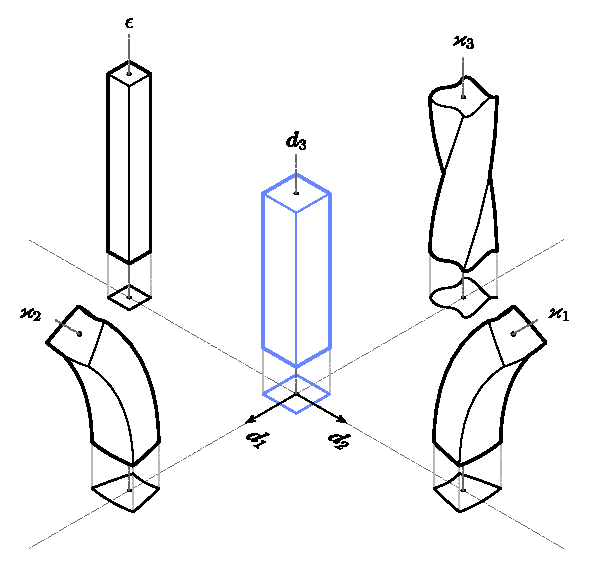
\includegraphics[]{kirchhoff_cross_section_deformation.pdf}
	\captionof{figure}[Typical deformation modes of cross-sections in Kirchhoff's theory]{Typical deformation modes of cross-sections in Kirchhoff's theory. Flexion around $\vect{d}_1$ (resp. $\vect{d}_2$) is measured through the material curvature $\varkappa_1$ (resp. $\varkappa_2$) ; torsion around $\vect{d}_3$ is measured through the material twist $\varkappa_3$ ; and $\epsilon$ measures the axial extension. Remark that cross-sections are subjected to both in-plane deformations ($\varkappa_1$, $\varkappa_2$, $\epsilon$) and out-of-plane deformations ($\varkappa_3$).}
	\label{fig:section_defo}
	\end{fullpage}
\end{figure}
In this paragraph, we simply recall the canonical form of the local displacement field ($\vect{u}$) for the cross-section $\mathcal{S}(s)$ in the context of Kirchhoff's approximation~: \footnote{Remark that the local displacement field results from the superposition of the three displacement fields obtained for pure and uniform extension, flexion and twist. For a detailed analysis of pure and uniform flexion and twist of rods refer to~\cite[ch.~3]{Audoly2010}.}
\begin{subequations}
	\begin{alignat}{1}
	u_3 &= (\varkappa_3 - \rconf{\varkappa}_3)\varphi_s(X_1,X_2)
	\\[0.5em]
	u_1 &=
	-\nu \epsilon X_1 
	- \nu(\varkappa_1 - \rconf{\varkappa}_1) X_1 X_2
	+ \tfrac{1}{2}\nu(\varkappa_2 - \rconf{\varkappa}_2)({X_1}^2 - {X_2}^2)
	\\[0.5em]
	u_2 &= 
	-\nu \epsilon X_2 
	+ \nu(\varkappa_2 - \rconf{\varkappa}_2) X_1 X_2
	+ \tfrac{1}{2}\nu(\varkappa_1 - \rconf{\varkappa}_1)({X_1}^2 - {X_2}^2)
	\end{alignat}
\end{subequations}
where $\varphi_s$ is the warping function in torsion of $\mathcal{S}(s)$, determined by the following differential equation and the boundary condition over the contour of the cross-section~: \footnote{\blockcquote{Campanile2009}{In the traditional theory of non-uniform torsion the axial displacement field is expressed as the product of the unit twist angle and the warping function. The first one, variable along the beam axis, is obtained by a global congruence condition; the second one, instead, defined over the cross-section, is determined by solving a Neumann problem associated to the Laplace equation, as well as for the uniform torsion problem.}.}\textsuperscript{,}\footnote{$\vect{n} = ({\partial f_s}/{\partial {X_1}}, {\partial f_s}/{\partial {X_1}})^T$ is the unit normal vector to the boundary curve of $\mathcal{S}(s)$ defined implicitly by the equation $f_s(X_1,X_2)=0$.}
\begin{subequations}
	\begin{alignat}{5}
	0 &= \frac{\partial^2 \varphi_s}{\partial {X_1}^2} + \frac{\partial^2 \varphi_s}{\partial {X_2}^2}
	&&  \quad, \quad \forall (X_1,X_2)\in\mathcal{S}(s)
	\\[0.5em]
	0 &= \frac{\partial f_s}{\partial {X_1}}\left(\frac{\partial \varphi_s}{\partial {X_1}} - X_2 \right) 
	+ \frac{\partial f_s}{\partial {X_2}}\left(\frac{\partial \varphi_s}{\partial {X_2}} + X_1 \right)
	&& \quad, \quad f_s(X_1,X_2) = 0 \label{eq:warpingCL}
	\end{alignat}
\end{subequations}
These equations have known analytical solutions for classical shapes such as circles, ellipses, squares or rectangles. For other shapes, when it is not easy to find analytical solutions, the membrane analogy introduced by \citef{Prandtl1903} can be employed.\footnote{Recent advances~\cite{Koohestani2014} in the form-finding of soap films with the force density method might be of practical use to evaluate the warping function.} A careful introduction to the question of torsion in bars is proposed by \citef[p.~258-315]{Timoshenko1951}.

Note that the boundary condition given by \cref{eq:warpingCL} stipulates that cross-sections are free to warp. The problem is more complex when warping is restrained. In this case, called \emph{non-uniform torsion}, the twisting stiffness is modified.\footnote{\blockcquote{Timoshenko1945b}{The problem becomes more complicated if cross sections are not free to warp or if the torque varies along the length of the bar. Warping in such cases varies along the bar and torsion is accompanied by tension or compression of longitudinal fibers. The rate of change of the angle of twist along the axis of the bar also varies, and we call this the case of non-uniform torsion.}.}

To go further on the subject of non uniform torsion, which is not treated in the present work, the reader is invited to refer to \cite{Vlasov1961,Elter1984,Alves2014}.

\subsection{Strain tensor}
Here, we remind the canonical form of the strain tensor ($\tens{E}$) for the cross-section $\mathcal{S}(s)$ in the context of Kirchhoff's approximation~: 
\begin{subequations}
	\begin{alignat}{1}
	\epsilon_{33} &= \epsilon + (\varkappa_1 - \rconf{\varkappa}_1) X_2 - (\varkappa_2 - \rconf{\varkappa}_2) X_1 \label{eq:strain_a}
	\\
	\epsilon_{11} &=  \epsilon_{22} = -\nu \epsilon_{33}	\label{eq:strain_b}
	\\
	\epsilon_{12} &= 0 \label{eq:strain_c}
	\\
	\epsilon_{31} &= \tfrac{1}{2}(\varkappa_3 - \rconf{\varkappa}_3)\left(\frac{\partial \varphi_s}{\partial {X_1}} - X_2 \right) \label{eq:strain_d}
	\\
	\epsilon_{32} &= \tfrac{1}{2}(\varkappa_3 - \rconf{\varkappa}_3)\left(\frac{\partial \varphi_s}{\partial {X_2}} + X_1 \right) \label{eq:strain_e}
	\end{alignat}
\end{subequations}

\subsection{Stress tensor}
In this paragraph, we simply give the entries of the stress tensor ($\tens{S}$) defined in \cref{eq:Stensor}, for the cross-section $\mathcal{S}(s)$ in the context of Kirchhoff's approximation~: 
\begin{subequations}
	\begin{alignat}{1}
	\sigma_{33} &= E \epsilon_{33} \label{eq:stress_a}
	\\
	\sigma_{11} &=  \sigma_{22} = \sigma_{12} = 0 \label{eq:stress_b}
	\\
	\sigma_{31} &= 2G \epsilon_{31}	\label{eq:stress_c}
	\\
	\sigma_{32} &= 2G \epsilon_{32}	\label{eq:stress_d}
	\end{alignat}
\end{subequations}
Thus, the Piola stress vector defined in \cref{eq:piola} becomes~:
\begin{equation}
	\vect{\sigma_n} = \sigma_{31}\vect{d}_1 + \sigma_{32}\vect{d}_2 + \sigma_{33}\vect{d}_3 \label{eq:piola2}
\end{equation}

\subsection{Constitutive equations for internal forces and moments}\label{sec:constit}
In Kirchhoff's theory, constitutive equations for internal forces and moments should not be considered as assumptions. Indeed, as shown hereafter, they are somehow consequences of the assumptions made on the motion -- that is the rod remains close to a motion where cross-sections remain planar, undistorted and perpendicular to the centerline -- and on the material -- the Hookean elasticity -- of the rod.

From \cref{eq:F,eq:piola2,eq:stress_a,eq:strain_a} we deduce the constitutive equation for the axial component of the internal forces~: \footnote{Also recall from \cref{eq:centroid} that $\iint_{\mathcal{S}(s)} {X_1} \;dX_1 dX_2 = 0$ and $\iint_{\mathcal{S}(s)} {X_2} \;dX_1 dX_2 = 0$.}
\begin{equation}
%	\label{eq:constitutive_F3}
	\begin{aligned}
		F_3 &= \iint_{\mathcal{S}(s)} \vect{\sigma_n}(s, X_1, X_2, t) \cdot \vect{d}_3 \;dX_1 dX_2 
		\\[0.5em]
		&= ES\epsilon 
		- (\varkappa_2 - \rconf{\varkappa}_2) \iint_{\mathcal{S}(s)} {X_1} \;dX_1 dX_2
		+ (\varkappa_1 - \rconf{\varkappa}_1) \iint_{\mathcal{S}(s)} {X_2} \;dX_1 dX_2
		\\[0.5em]
		&= ES\epsilon
	\end{aligned}
\end{equation}
From \cref{eq:M,eq:piola2,eq:stress_c,eq:stress_d,eq:strain_e,eq:strain_d} we deduce the constitutive equation for the axial component of the internal moments, that is the twisting moment~: 
\begin{equation}
% 	\label{eq:constitutive_M3}
	\begin{aligned}
		M_3 &= \iint_{\mathcal{S}(s)} (\vect{r} \times \vect{\sigma_n}(s, X_1, X_2, t)) \cdot \vect{d}_3 \;dX_1 dX_2
		\\[0.5em]
		&= \iint_{\mathcal{S}(s)} \big[-X_2\sigma_{31} + X_1\sigma_{32} \big] \;dX_1 dX_2 
		\\[0.5em]
		&= G (\varkappa_3 - \rconf{\varkappa}_3) 
		\iint_{\mathcal{S}(s)} \Big[ X_1 \left( \frac{\partial \varphi_s}{\partial {X_2}} + X_1 \right ) - X_2 \left( \frac{\partial \varphi_s}{\partial {X_1}}  - X_2 \right )
		 \Big] \;dX_1 dX_2 
	\end{aligned}
\end{equation}
Introducing the torsional constant of St Venant ($J$) this equation rewrites~:
\begin{subequations}
	\begin{alignat}{2}
	M_3 &= GJ (\varkappa_3 - \rconf{\varkappa}_3)
	\\
	J &= \iint_{\mathcal{S}(s)} \Big[ X_1 \left( \frac{\partial \varphi_s}{\partial {X_2}} + X_1 \right ) - X_2 \left( \frac{\partial \varphi_s}{\partial {X_1}}  - X_2 \right )
		 \Big] \;dX_1 dX_2 \label{eq:torsioncst_def}
	\end{alignat}
\end{subequations}
Remark from \cref{eq:torsioncst_def} that when the section does not warp ($\varphi_s$=0), the torsion constant is nothing but the polar moment of inertia of the section ($I_p$).

From \cref{eq:M,eq:piola2,eq:stress_a,eq:strain_a} we deduce the constitutive equation for the first component of the internal moments~: 
\begin{equation}
% 	\label{eq:constitutive_M3}
	\begin{aligned}
		M_1 &= \iint_{\mathcal{S}(s)} (\vect{r} \times \vect{\sigma_n}(s, X_1, X_2, t)) \cdot \vect{d}_1 \;dX_1 dX_2
		\\[0.5em]
		&= \iint_{\mathcal{S}(s)} X_2\sigma_{33} \;dX_1 dX_2 
		\\[0.5em]
		&= E (\varkappa_1 - \rconf{\varkappa}_1) \iint_{\mathcal{S}(s)} {X_2}^2  \;dX_1 dX_2 
	\end{aligned}
\end{equation}
From \cref{eq:M,eq:piola2,eq:stress_a,eq:strain_a} we deduce the constitutive equation for the second component of the internal moments~: 
\begin{equation}
% 	\label{eq:constitutive_M3}
	\begin{aligned}
		M_2 &= \iint_{\mathcal{S}(s)} (\vect{r} \times \vect{\sigma_n}(s, X_1, X_2, t)) \cdot \vect{d}_2 \;dX_1 dX_2
		\\[0.5em]
		&= \iint_{\mathcal{S}(s)} - X_1\sigma_{33} \;dX_1 dX_2 
		\\[0.5em]
		&= E (\varkappa_2 - \rconf{\varkappa}_2) \iint_{\mathcal{S}(s)} {X_1}^2  \;dX_1 dX_2 
	\end{aligned}
\end{equation}

\subsection{Discussion}
Observe that the internal shear forces are reacting parameters and are given by the balance equations (see \cref{eq:motion_4,eq:motion_5}). Transverse shear deformations are neglected and the related stresses are not given by the present theory.

Cross-sections are not assumed to be subject to rigid body motions but to deform closely to such movements. Indeed, the torsion constant of St Venant ($J$) is found assuming the cross-sections can warp (see \cref{eq:torsioncst}). Otherwise, the constant torsion would be nothing but the polar moment of inertia, which would not lead to the correct evaluation of the torsional stiffness of the rod.

Because of the chosen description of motion (see \cref{sec:kirchhoff_motion}), cross-sections are assumed to rotate around their center of mass. Hence, the model is only valid for sections where the shear center is located at the center of mass. This preclude thin walled open cross-sections. For further understanding of the warping of sections, refer to \cite{Alves2014}.


%
%It is mandatory to suppose that sections can wrapped
%
%Warping is supposed to happen freely. 

%
%\item
%There is a noticeable symmetry in the equations between the roles played by $F_1$, $F_2$ and $M_1$, $M_2$ and by the roles played by $F_3$ and $M_3$.
%\item
%Warping is supposed to happen freely.
%\item
%Going further with torsion : donner des citations
%\item
%Going further with shear and extension : \cite{Reissner1973}
%\end{itemize}

\clearpage
\section{Summary of Kirchhoff theory}\label{sec:ksummary}
Let's summarize the assumptions and results of Kirchhoff's theory of rods on which our discret beam model (see \cref{chp:numerical_model}) will be based on.

In the reference configuration the rod is described by its reference strains~:
\begin{equation}
	\rconf{\vect{d}_i}'= \rconf{\vect{\varkappa}}  \times \rconf{\vect{d}_i}
\end{equation}
In the actual configuration the rod is described by its strain and spin vectors~:
\begin{subequations}
	\begin{alignat}{1}
	\vect{x}' &= (1+\epsilon)\vect{t}
	\\
	\vect{d}'_i&= {\vect{\varkappa}}  \times \vect{d}_i
	\\
	\dot{\vect{d}_i}&= {\vect{\omega}}  \times \vect{d}_i
	\end{alignat}
\end{subequations}
The rod is subjected to internal forces and moments~:
\begin{subequations}
	\begin{alignat}{1}
	\vect{F} &= F_1\vect{d}_1 + F_2\vect{d}_2 + F_3\vect{d}_3
	\\
	\vect{M} &= M_1\vect{d}_1 + M_2\vect{d}_2 + M_3\vect{d}_3
	\end{alignat}
\end{subequations}
The rod is subjected to external and body loads described as distributed forces and moments acting on the centerline -- either given per unit length of the reference configuration ($\vect{f}_{s} $, $\vect{m}_{s} $) or per unit length of the actual configuration ($\vect{f}_{s_t}$, $\vect{m}_{s_t} $) -- and given by~:
\begin{subequations}
	\begin{alignat}{1}
	\vect{f} &= \vect{f}_{s}  + (1+\epsilon)\vect{f}_{s_t} = f_1\vect{d}_1 + f_2\vect{d}_2 + f_3\vect{d}_3
	\\
	\vect{m} &= \vect{m}_{s}  + (1+\epsilon)\vect{m}_{s_t}  = m_1\vect{d}_1 + m_2\vect{d}_2 + m_3\vect{d}_3
	\end{alignat}
\end{subequations}
The internal axial force, the internal bending moments and the internal twisting moment are computed with the following constitutive equations~:
\begin{subequations}
	\begin{alignat}{1}
	F_3 &= ES\epsilon \label{eq:constitutive_a}
	\\
	M_1 &= EI_1(\varkappa_1 - \rconf{\varkappa}_1) \label{eq:constitutive_b}
	\\
	M_2 &= EI_2(\varkappa_2 - \rconf{\varkappa}_2) \label{eq:constitutive_c}
	\\
	M_3 &= GJ(\varkappa_3 - \rconf{\varkappa}_3) \label{eq:constitutive_d}
	\end{alignat}
\end{subequations}
where $S$, $I_1$, $I_2$, $J$ are respectively the area, the second moments of inertia and the torsional stiffness of the cross-section~:
\begin{subequations}
	\begin{alignat}{2}
	&S 	&&= \iint_{\mathcal{S}(s)} dX_1 dX_2
	\\
	&I_1	&&= \iint_{\mathcal{S}(s)} {X_2}^2 \;dX_1 dX_2
	\\
	&I_2	&&= \iint_{\mathcal{S}(s)} {X_1}^2 \;dX_1 dX_2
	\\
	&J 	&&= \iint_{\mathcal{S}(s)} X_1 \left( \frac{\partial \varphi_s}{\partial {X_2}} + X_1 \right ) - X_2 \left( \frac{\partial \varphi_s}{\partial {X_1}}  - X_2 \right )
			\;dX_1 dX_2 \label{eq:torsioncst}
	\end{alignat}
\end{subequations}
and $\varphi_s$ is the warping fonction of the cross-section that satisfies the differential system~: 
\begin{subequations}
	\begin{alignat}{2}
	0 &= \frac{\partial^2 \varphi_s}{\partial {X_1}^2} + \frac{\partial^2 \varphi_s}{\partial {X_2}^2}
	&&\quad,\quad \forall (X_1,X_2)\in\mathcal{S}(s)
	\\[0.5em]
	0 &= \frac{\partial f_s}{\partial {X_1}}\left(\frac{\partial \varphi_s}{\partial {X_1}} - X_2 \right) 
	+ \frac{\partial f_s}{\partial {X_2}}\left(\frac{\partial \varphi_s}{\partial {X_2}} + X_1 \right)
	&&\quad,\quad f_s(X_1,X_2) = 0
	\end{alignat}
\end{subequations}
The dynamical equations for the motion of the rod are~:
\begin{subequations}
	\begin{alignat}{1}
	\frac{\partial \vect{F}}{\partial s} + \vect{f} 
	&= \rho S \ddot{\vect{x}}
	\\[0.5em]
	\frac{\partial \vect{M}}{\partial s} 
	+ \frac{\partial \vect{x}}{\partial s} \times \vect{F}
	+ \vect{m} 
	&= \rho I_1 \vect{d}_1 \times \ddot{\vect{d}_1} + \rho I_2 \vect{d}_2 \times \ddot{\vect{d}_2}
	\end{alignat}
\end{subequations}
Neglecting the rotational dynamics around $\vect{d}_1$ and $\vect{d}_2$ the components of the above equations are written~:
\begin{subequations}
	\begin{alignat}{1}
	F'_1 + \varkappa_2 F_3 - \varkappa_3 F_2 + f_1 &= \rho S \ddot{x}_1  \label{eq:motion_1}
	\\
	F'_2 + \varkappa_3 F_1 - \varkappa_1 F_3 + f_2 &= \rho S \ddot{x}_2 \label{eq:motion_2}
	\\
	F'_3 + \varkappa_1 F_2 - \varkappa_2 F_1 + f_3 &= \rho S \ddot{x}_3 \label{eq:motion_3}
	\\
	M'_1 + \varkappa_2 M_3 - \varkappa_3 M_2 - (1+\epsilon)F_2  + m_1 & \simeq 0 \label{eq:motion_4}
	\\
	M'_2 + \varkappa_3 M_1 - \varkappa_1 M_3 + (1+\epsilon)F_1 + m_2 & \simeq 0 \label{eq:motion_5}
	\\
	M'_3 + \varkappa_1 M_2 - \varkappa_2 M_1 + m_3 & \simeq \rho (I_1 + I_2)\dot{\omega}_3 \label{eq:motion_6}
	\end{alignat}
	 \label{eq:motion}
\end{subequations}
The local displacements of the cross-sections are given by~:
\begin{subequations}
	\begin{alignat}{1}
	u_3 &= (\varkappa_3 - \rconf{\varkappa}_3)\varphi_s(X_1,X_2)
	\\[0.5em]
	u_1 &=
	-\nu \epsilon X_1 
	- \nu(\varkappa_1 - \rconf{\varkappa}_1) X_1 X_2
	+ \tfrac{1}{2}\nu(\varkappa_2 - \rconf{\varkappa}_2)({X_1}^2 - {X_2}^2)
	\\[0.5em]
	u_2 &= 
	-\nu \epsilon X_2 
	+ \nu(\varkappa_2 - \rconf{\varkappa}_2) X_1 X_2
	+ \tfrac{1}{2}\nu(\varkappa_1 - \rconf{\varkappa}_1)({X_1}^2 - {X_2}^2)
	\end{alignat}
\end{subequations}
The non-zero components of the strain tensor are given by~:
\begin{subequations}
	\begin{alignat}{1}
	\epsilon_{33} &= \epsilon + (\varkappa_1 - \rconf{\varkappa}_1) X_2 - (\varkappa_2 - \rconf{\varkappa}_2) X_1
	\\
	\epsilon_{31} &= \tfrac{1}{2}(\varkappa_3 - \rconf{\varkappa}_3)\left(\frac{\partial \varphi_s}{\partial {X_1}} - X_2 \right)
	\\
	\epsilon_{32} &= \tfrac{1}{2}(\varkappa_3 - \rconf{\varkappa}_3)\left(\frac{\partial \varphi_s}{\partial {X_2}} + X_1 \right)
	\\
	\epsilon_{11} &=  \epsilon_{22} = -\nu \epsilon_{33}
	\end{alignat}
\end{subequations}
The non-zero components of the stress tensor are given by~:
\begin{subequations}
	\begin{alignat}{1}
	\sigma_{33} &= E \epsilon_{33} 
	\\
	\sigma_{31} &= 2G \epsilon_{31}
	\\
	\sigma_{32} &= 2G \epsilon_{32}
	\end{alignat}
\end{subequations}






%\makebox[\textwidth]{} % necessaire pour le saut de page et le flush des floats
%\newpage
\section{Geometric interpretation of Kirchhoff's equations}\label{sec:geointerp}

The previous equations for the motion of the rod have been established expressing the fundamental principles of balance of linear and angular momentums (see \cref{eq:motion_1,eq:motion_2,eq:motion_3,eq:motion_4,eq:motion_5,eq:motion_6}). An alternative approach, leading to the same results, consists in differentiating the elastic energy of a given configuration of the rod -- assumed to be stationary -- with respect to the degrees of freedom of the mechanical system (principle of virtual work). This latter approach is the one developed throughout the previous chapter (see \cref{chp:energy}).\footnote{This is also the approach developed by \citef{Audoly2010} for strictly inextensible rods. It was yet employed by \citef{Reissner1973}.} 

However, the approach through equilibrium seems easier to understand as it is (almost) just a matter of balance between forces and moments acting on infinitesimal slices of the rods (see \cref{fig:slice}). This is of obvious pedagogical interest as it allows to understand how the geometry of the rod influences the distribution of the elastic energy between extension, flexion and torsion and how these forces are coupled together.

To emphasis this, in this section we provide the proper drawings (see \cref{fig:kb,fig:d1,fig:d2}) and computations for the contribution of internal forces and moments to the balance of linear and angular momentums. This is what we call here the \textquote{geometric interpretation} of Kirchhoff equations.
\begin{figure}[p]
  \begin{fullpage}
	\centering
	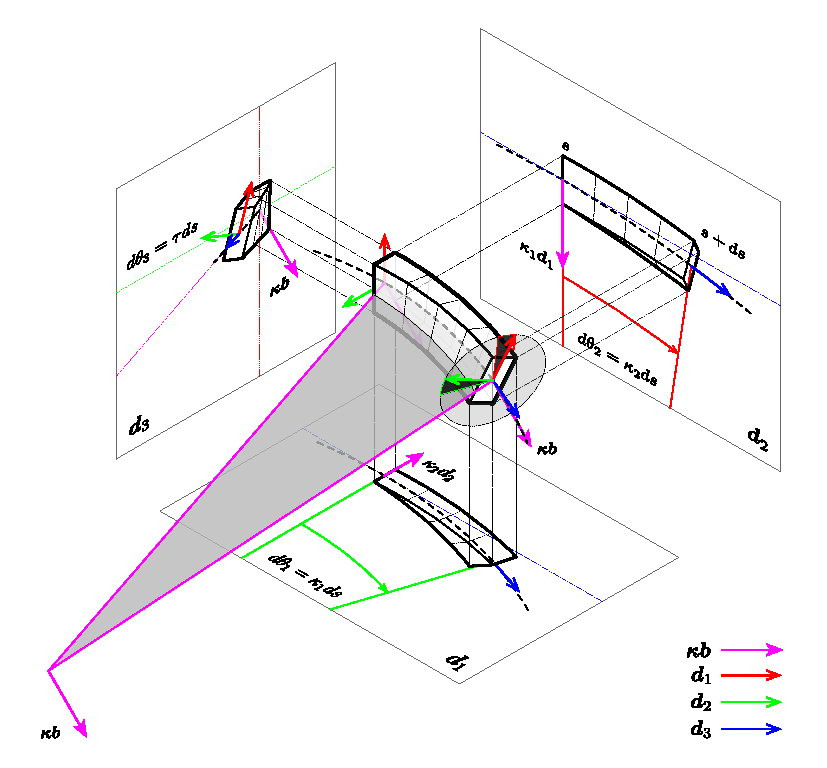
\includegraphics[]{kirchhoff_geometry.pdf}
	\captionof{figure}[Geometric interpretation of Kirchhoff's equations]{Geometric interpretation of Kirchhoff's equations. Flexion and torsion of an elementary slice of a Kirchhoff rod of length $ds$. Projections of the deformations are given in the material planes perpendicular to $\vect{d}_1$, $\vect{d}_2$ and $\vect{d}_3$. The element takes its curvature $\kappa$ in the plane perpendicular to $\vect{\kappa b}$ and represented by a gray triangle. On the figure, $\vect{\kappa b}$ is positioned at the peak of this triangle, which is the center of the osculating circle associated to it.}
	\label{fig:slice}
 \end{fullpage}
\end{figure} 
\begin{figure}[p]
  \begin{leftfullpage}
    \captionsetup[subfloat]{captionskip=10pt}
     	\centering
     	\subfloat[][infinitesimal deformation]{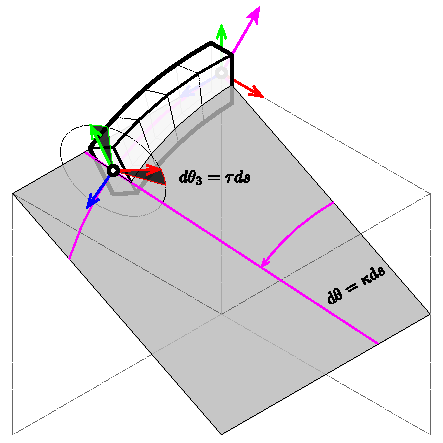
\includegraphics{kirchhoff_geometry_kb.pdf}\label{fig:kb_a}} \\
	\vspace{30pt}
	\subfloat[][contributions of the internal forces]{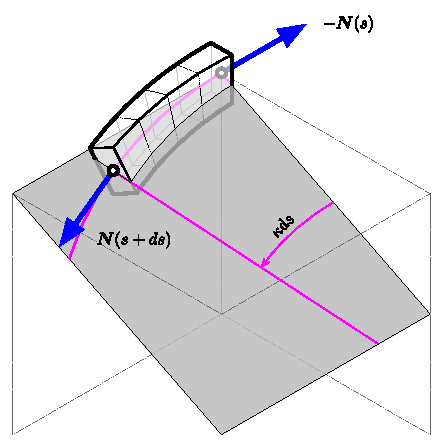
\includegraphics{kirchhoff_balance_T_kb.pdf}\label{fig:kb_b}}
	\subfloat[][contributions of the internal moments]{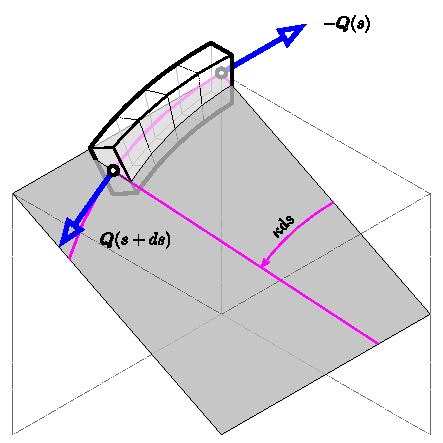
\includegraphics{kirchhoff_balance_M_kb.pdf}\label{fig:kb_c}}
	\vspace{30pt}
	\captionof{figure}[Interpretation~: influence of the curvature ($\kappa$)]{Influence of the curvature ($\kappa$) in the deflection of internal forces and moments along the centerline. The osculating plane, perpendicular to $\vect{\kappa b}$, is represented in grey. $\vect{N}$ is the axial component of the internal force along $\vect{d}_3$. $\vect{Q}$ is the axial component of the internal moment, also known as the twisting moment along $\vect{d}_3$.}     
	\label{fig:kb}
 \end{leftfullpage}
\end{figure}
\begin{figure}[p]
	\begin{fullpage}
	\subsubsection{Contributions to the balance of forces}
	\vspace{10pt}
	$\vect{N}(s+ds)$ is deflected from $\vect{d}_3(s)$ by the rotation of angle $\kappa ds$ around $\vect{\kappa b}$ (\cref{fig:kb_b}). Thus, its contribution to the balance of forces onto $\vect{d}_3(s)$ is~: 
	\begin{equation*}
		N(s+ds) \cos(\kappa ds) - N(s) = N'(s) ds + o(ds)
	\end{equation*}	
	\vspace{10pt}
	
	\subsubsection{Contributions to the balance of moments}
	\vspace{10pt}
	$\vect{Q}(s+ds)$ is deflected from $\vect{d}_3(s)$ by the rotation of angle $\kappa ds$ around $\vect{\kappa b}$ (\cref{fig:kb_c}). Thus, its contribution to the balance of moments onto $\vect{d}_3(s)$ is~: 
	\begin{equation*}
		Q(s+ds) \cos(\kappa ds) - Q(s) = Q'(s) ds + o(ds)
	\end{equation*}	
	  \end{fullpage}
\end{figure}

% ============
 
\begin{figure}[p]
  \begin{leftfullpage}
    \captionsetup[subfloat]{captionskip=10pt}
     	\centering
     	\subfloat[][infinitesimal deformation]{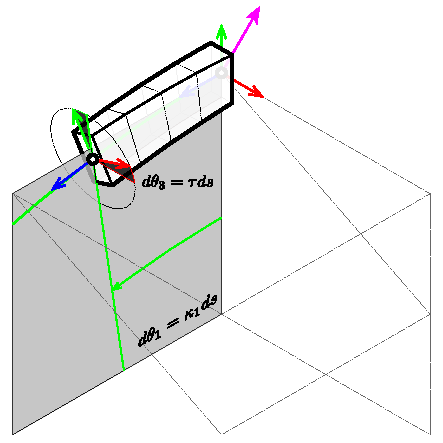
\includegraphics{kirchhoff_geometry_d1.pdf}\label{fig:d1_a}} \\
	\vspace{30pt}
	\subfloat[][contributions of the internal forces]{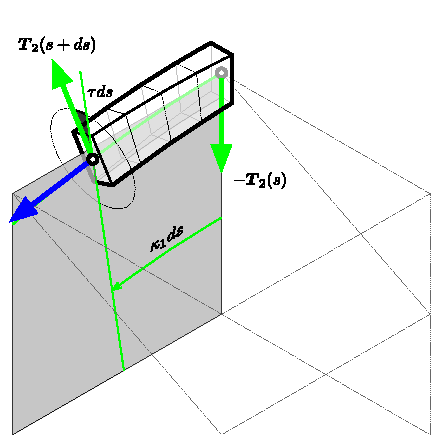
\includegraphics{kirchhoff_balance_T_d1.pdf}\label{fig:d1_b}}
	\subfloat[][contributions of the internal moments]{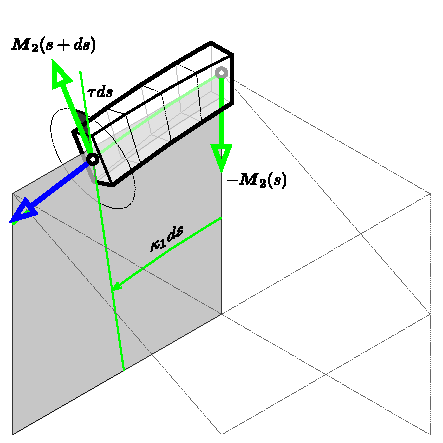
\includegraphics{kirchhoff_balance_M_d1.pdf}\label{fig:d1_c}}
	\vspace{30pt}
	\captionof{figure}[Interpretation~: influence of the first material curvature ($\kappa_1$)]{Influence of the first material curvature ($\kappa_1$) in the deflection of internal forces and moments along the centerline. The plane perpendicular to $\vect{d}_1(s)$ is represented in grey. $\vect{F}_2$ is the transverse or shear component of the internal force along $\vect{d}_2$. $\vect{M}_2$ is the transverse or bending component of the internal moment along $\vect{d}_2$.}     
	\label{fig:d1}
 \end{leftfullpage}
\end{figure}
\begin{figure}[p]
	\begin{fullpage}
	\subsubsection{Contributions to the balance of forces}
	\vspace{10pt}
	
	$\vect{F}_2(s+ds)$ is deflected from $\vect{d}_2(s)$ by the combined rotations of angle $\tau ds$ around $\vect{d}_3$ and $\kappa_2 ds$ around $\vect{d}_2$ (\cref{fig:d1_b}). Thus, its contribution to the balance of forces onto $\vect{d}_1(s)$ is~: 
	\begin{equation*}
		-F_2(s+ds) \sin(\tau ds) \cos(\kappa_2 ds) = -\tau F_2(s) ds + o(ds)
	\end{equation*}	
	
	$\vect{F}_2(s+ds)$ is deflected from $\vect{d}_2(s)$ by the combined rotations of angle $\tau ds$ around $\vect{d}_3$ and $\kappa_1 ds$ around $\vect{d}_1$ (\cref{fig:d1_b}). Thus, its contribution to the balance of forces onto $\vect{d}_2(s)$ is~: 
	\begin{equation*}
		-F_2(s) + F_2(s+ds) \cos(\tau ds) \cos(\kappa_1 ds) = F'_2 (s) ds + o(ds)
	\end{equation*}	
	
	$\vect{F}_2(s+ds)$ is deflected from $\vect{d}_2(s)$ by the combined rotations of angle $\tau ds$ around $\vect{d}_3$ and $\kappa_1 ds$ around $\vect{d}_1$ (\cref{fig:d1_b}). Thus, its contribution to the balance of forces onto $\vect{d}_3(s)$ is~: 
	\begin{equation*}
		F_2(s+ds) \cos(\tau ds) \sin(\kappa_1 ds) = \kappa_1 F_2(s) ds + o(ds)
	\end{equation*}
		
	$\vect{N}(s+ds)$ is deflected from $\vect{d}_3(s)$ by the combined rotations of angle $\kappa_2 ds$ around $\vect{d}_2$ and $\kappa_1 ds$ around $\vect{d}_1$ (\cref{fig:d1_b}). Thus, its contribution to the balance of forces onto $\vect{d}_2(s)$ is~: 
	\begin{equation*}
		-N(s+ds) \cos(\kappa_2 ds) \sin(\kappa_1 ds) = -\kappa_1 N(s) ds + o(ds)
	\end{equation*}	
	\vspace{10pt}

	\subsubsection{Contributions to the balance of moments}
	\vspace{10pt}
	
	$\vect{F}_2(s+ds)$ is deflected from the plane normal to $\vect{d}_1(s)$ by a rotation of angle $\tau ds$ around $\vect{d}_3$ (\cref{fig:d1_b}). It produces a moment around $\vect{d}_1$ with the lever arm $b =  \cos(\kappa_2 ds) ds$. Thus, its contribution to the balance of moments onto $\vect{d}_1(s)$ is~: 
	\begin{equation*}
		-F_2(s+ds) \cos(\tau ds) (\cos(\kappa_2 ds) ds) = -F_2(s) ds + o(ds)
	\end{equation*}
	
	$\vect{M}_2(s+ds)$ is deflected from $\vect{d}_2(s)$ by the combined rotations of angle $\tau ds$ around $\vect{d}_3$ and $\kappa_2 ds$ around $\vect{d}_2$ (\cref{fig:d1_c}). Thus, its contribution to the balance of moments onto $\vect{d}_1(s)$ is~: 
	\begin{equation*}
		-M_2(s+ds) \sin(\tau ds) \cos(\kappa_2 ds) = -\tau M_2 (s) ds + o(ds)
	\end{equation*}	
	
	$\vect{M}_2(s+ds)$ is deflected from $\vect{d}_2(s)$ by the combined rotations of angle $\tau ds$ around $\vect{d}_3$ and $\kappa_1 ds$ around $\vect{d}_1$ (\cref{fig:d1_c}). Thus, its contribution to the balance of moments onto $\vect{d}_2(s)$ is~: 
	\begin{equation*}
		-M_2(s) + M_2(s+ds) \cos(\tau ds) \cos(\kappa_1 ds) = M'_2 (s) ds + o(ds)
	\end{equation*}
	
	$\vect{M}_2(s+ds)$ is deflected from $\vect{d}_2(s)$ by the combined rotations of angle $\tau ds$ around $\vect{d}_3$ and $\kappa_1 ds$ around $\vect{d}_1$ (\cref{fig:d1_c}). Thus, its contribution to the balance of moments onto $\vect{d}_3(s)$ is~: 
	\begin{equation*}
		M_2(s+ds) \cos(\tau ds) \sin(\kappa_1 ds) = \kappa_1 M_2 (s) ds + o(ds)
	\end{equation*}	
	
	$\vect{Q}(s+ds)$ is deflected from $\vect{d}_3(s)$ by the combined rotations of angle $\kappa_2 ds$ around $\vect{d}_2$ and $\kappa_1 ds$ around $\vect{d}_1$ (\cref{fig:d1_c}). Thus, its contribution to the balance of moments onto $\vect{d}_2(s)$ is~: 
	\begin{equation*}
		-Q(s+ds) \cos(\kappa_2 ds) \sin(\kappa_1 ds) = -\kappa_1 Q(s) ds + o(ds)
	\end{equation*}	
	  \end{fullpage}
\end{figure}

% ============
 
\begin{figure}[p]
  \begin{leftfullpage}
    \captionsetup[subfloat]{captionskip=10pt}
     	\centering
     	\subfloat[][infinitesimal deformation]{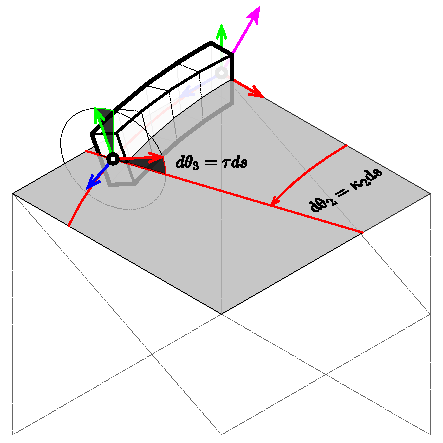
\includegraphics{kirchhoff_geometry_d2.pdf}\label{fig:d2_a}} \\
	\vspace{30pt}
	\subfloat[][contributions of the internal forces]{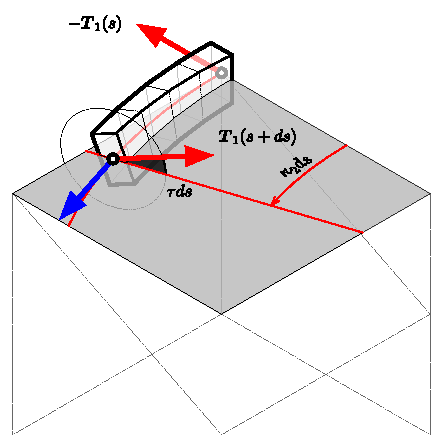
\includegraphics{kirchhoff_balance_T_d2.pdf}\label{fig:d2_b}}
	\subfloat[][contributions of the internal moments]{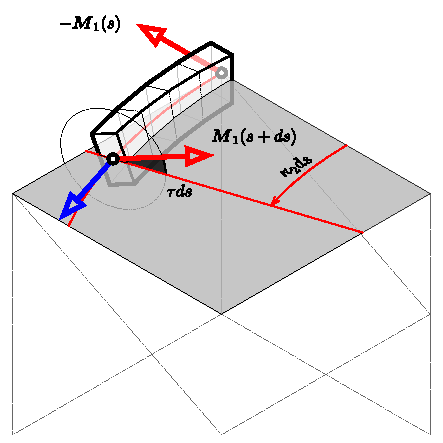
\includegraphics{kirchhoff_balance_M_d2.pdf}\label{fig:d2_c}}
	\vspace{30pt}
	\captionof{figure}[Interpretation~: influence of the second material curvature ($\kappa_2$)]{Influence of the second material curvature ($\kappa_2$) in the deflection of internal forces and moments along the centerline. The plane perpendicular to $\vect{d}_2(s)$ is represented in grey. $\vect{F}_1$ is the transverse or shear component of the internal force along $\vect{d}_1$. $\vect{M}_1$ is the transverse or bending component of the internal moment along $\vect{d}_1$.}     
	\label{fig:d2}
 \end{leftfullpage}
\end{figure}
\begin{figure}[p]
	\begin{fullpage}
	\subsubsection{Contributions to the balance of forces}
	\vspace{10pt}
	
	$\vect{F}_1(s+ds)$ is deflected from $\vect{d}_1(s)$ by the combined rotations of angle $\tau ds$ around $\vect{d}_3$ and $\kappa_2 ds$ around $\vect{d}_2$ (\cref{fig:d2_b}). Thus, its contribution to the balance of forces onto $\vect{d}_1(s)$ is~: 
	\begin{equation*}
		-F_1(s) + F_1(s+ds) \cos(\tau ds) \cos(\kappa_2 ds) = F'_1 (s) ds + o(ds)
	\end{equation*}
	
	$\vect{F}_1(s+ds)$ is deflected from $\vect{d}_1(s)$ by the combined rotations of angle $\tau ds$ around $\vect{d}_3$ and $\kappa_1 ds$ around $\vect{d}_1$ (\cref{fig:d2_b}). Thus, its contribution to the balance of forces onto $\vect{d}_2(s)$ is~: 
	\begin{equation*}
		F_1(s+ds) \sin(\tau ds) \cos(\kappa_1 ds) = \tau F_1 (s) ds + o(ds)
	\end{equation*}	
	
	$\vect{F}_1(s+ds)$ is deflected from $\vect{d}_1(s)$ by the combined rotations of angle $\tau ds$ around $\vect{d}_3$ and $\kappa_2 ds$ around $\vect{d}_2$ (\cref{fig:d2_b}). Thus, its contribution to the balance of forces onto $\vect{d}_3(s)$ is~: 
	\begin{equation*}
		-F_1(s+ds) \cos(\tau ds) \sin(\kappa_2 ds) = - \kappa_2 F_1(s) ds + o(ds)
	\end{equation*}	
	
	$\vect{N}(s+ds)$ is deflected from $\vect{d}_3(s)$ by the combined rotations of angle $\kappa_1 ds$ around $\vect{d}_1$ and $\kappa_2 ds$ around $\vect{d}_2$ (\cref{fig:d2_b}). Thus, its contribution to the balance of forces onto $\vect{d}_1(s)$ is~: 
	\begin{equation*}
		N(s+ds) \cos(\kappa_1 ds) \sin(\kappa_2 ds) = \kappa_2 N(s) ds + o(ds)
	\end{equation*}
	\vspace{10pt}

	\subsubsection{Contributions to the balance of moments}
	\vspace{10pt}
	
		$\vect{F}_1(s+ds)$ is deflected from the plane normal to $\vect{d}_2(s)$ by the angle $\tau ds$ around $\vect{d}_3$ along $ds$ (\cref{fig:d2_b}). It produces a moment around $\vect{d}_2$ with the lever arm $b =  \cos(\kappa_1 ds) ds$. Thus, its contribution to the balance of moments onto $\vect{d}_2(s)$ is~: 
	\begin{equation*}
		F_1(s+ds) \cos(\tau ds) (\cos(\kappa_1 ds) ds) = F_1(s) ds + o(ds)
	\end{equation*}
	
	$\vect{M}_1(s+ds)$ is deflected from $\vect{d}_1(s)$ by the combined rotations of angle $\tau ds$ around $\vect{d}_3$ and $\kappa_2 ds$ around $\vect{d}_2$ (\cref{fig:d2_c}). Thus, its contribution to the balance of moments onto $\vect{d}_1(s)$ is~: 
	\begin{equation*}
		-M_1(s) + M_1(s+ds) \cos(\tau ds) \cos(\kappa_2 ds) = M'_1 (s) ds + o(ds)
	\end{equation*}	
	
	$\vect{M}_1(s+ds)$ is deflected from $\vect{d}_1(s)$ by the combined rotations of angle $\tau ds$ around $\vect{d}_3$ and $\kappa_2 ds$ around $\vect{d}_2$ (\cref{fig:d2_c}). Thus, its contribution to the balance of moments onto $\vect{d}_2(s)$ is~: 
	\begin{equation*}
		M_1(s+ds) \sin(\tau ds) \cos(\kappa_2 ds) = \tau M_1 (s) ds + o(ds)
	\end{equation*}	
	
	$\vect{M}_1(s+ds)$ is deflected from $\vect{d}_1(s)$ by the combined rotations of angle $\tau ds$ around $\vect{d}_3$ and $\kappa_2 ds$ around $\vect{d}_2$ (\cref{fig:d2_c}). Thus, its contribution to the balance of moments onto $\vect{d}_3(s)$ is~: 
	\begin{equation*}
		-M_1(s+ds) \cos(\tau ds) \sin(\kappa_2 ds) = -\kappa_2 M_1 (s) ds + o(ds)
	\end{equation*}	
	
	$\vect{Q}(s+ds)$ is deflected from $\vect{d}_3(s)$ by the combined rotations of angle $\kappa_1 ds$ around $\vect{d}_1$ and $\kappa_2 ds$ around $\vect{d}_2$ (\cref{fig:d2_c}). Thus, its contribution to the balance of moments onto $\vect{d}_1(s)$ is~: 
	\begin{equation*}
		Q(s+ds) \cos(\kappa_1 ds) \sin(\kappa_2 ds) = \kappa_2 Q(s) ds + o(ds)
	\end{equation*}	
	  \end{fullpage}
\end{figure}

\clearpage
\section{Conclusion}
The geometric configuration of a Kirchhoff rod has been described using a constrained Cosserat rod model, composed of a centerline curve and an orthonormal adapted frame. The assumptions upon which Kirchhoff theory for rods is built has been carefully reminded and the dynamical equations of a rod has been established. A pure geometric reasoning has been proposed to retrieve the static member of these equations, understood as first order balance laws between internal force and moment.

These theoretical clarifications give a more robust understanding of the previous works of \citef{Adriaenssens1999}, \citef{Douthe2007} and \citef{DAmico2014} on nonlinear rod models for the computation of elastic gridshells. Indeed, we have shown that the material curvature is the one that comes up in the calculation of the bending moment through the constitutive laws and that it is distinct from the geometric curvature, although these notions could be considered equivalent in the case of weakly extensible rods. We have also demonstrated that the shear forces acting on the rod can be straightly deduced from the dynamical equations if the angular inertia around the material directors $\vect{d}_1$ and $\vect{d}_2$ is neglected. Finally, we have remarked that the equations of motion already take into account stretching, bending and twisting of the rod. Hence, the works previously developed in \cite{Adriaenssens1999,Douthe2007} about the \dofs{3} spline beam element are special cases of this set of dynamical equations.

In this chapter we have set up the theoretical basement to built a discrete rod model that is able to take into account axial extension, bending and torsion, and external loading. Previous works in this field can be understood as special cases of this framework and this enhance the overall understanding and the continuity between these works and the present thesis.

%The static member of these equations 
%
%We have draw up in a very different manner a new framework for the study of slender elastic rods in large displacement.
%
%+ proche de l'approche Barnes, Adriaenssens, Douthe
%+ physique / compréhension des memberes statiques comme des équilibres de force (suelement de la trigo !)
%+ hypothèses plus claires (pas d'inextensibilité, pas de quasistatique mais une assertion sur les moments d'inertie)
%+ clarifie la transposition du moment en couple d'effort proposé par Adrienssen, Doute, D'amico. Qu'"on comporend comme une équation d'éqiulibre statique.
%+ complète traitement naturel des charges appliquées


